\documentclass[letter,14pt]{extreport}
\usepackage[dvips]{graphicx}
%\usepackage{layout}
\bibliographystyle{osa_all_auth}
%\input{WEBBtemplate.sty}
\usepackage[square,comma,numbers,sort&compress]{natbib}
\usepackage{WEBBsmallbib}
\usepackage{mathrsfs}
\usepackage{wrapfig}
\usepackage{amsmath,amssymb,graphicx}
\usepackage{graphicx,color,hyperref,amsmath,units,float,abstract,tabulary,amsthm,amssymb,setspace}
\usepackage[margin=1.1in]{geometry}
\usepackage[titletoc]{appendix}
\usepackage[]{mcode}
\doublespacing
\newcommand{\sizetwelvefixed}{\fontsize{12}{14.4}\selectfont}

\usepackage{titlesec}
% \titleformat{\chapter}[display]% OLD
%     {\normalfont\huge\bfseries}{\chaptertitlename\ \thechapter}{20pt}{\Huge}% OLD
% \titlespacing*{\chapter}{0pt}{50pt}{40pt}% OLD
\titleformat{\chapter}[display]% NEW
    {\large\bfseries}{\chaptertitlename\ \thechapter}{5pt}{\Large}% NEW
\titlespacing*{\chapter}{0pt}{30pt}{20pt}% NEW

\begin{document}
\begin{titlepage}
\begin{center}
\textsc{\LARGE Purdue University}\\[1.0cm]
\textsc{\Large ECE513 Final Project}\\[1cm]
\hrule\hspace*{\fill}\\[0.8cm]
{\LARGE \bfseries Iterative Methods for
Diffractive Optical Element Design}\\[0.7cm]
\hrule\hspace*{\fill}\\[0.8cm]
\begin{minipage}{0.4\textwidth}
\hspace*{\fill}\\
\begin{flushleft} \large
\emph{Author:}\\
Qiaoen \textsc{Luo}\\
\end{flushleft}
\end{minipage}
\begin{minipage}{0.4\textwidth}
\hspace*{\fill}\\
\begin{flushright} \large
\emph{Supervisor:} \\
Prof.~Okan \textsc{Ersoy}
\end{flushright}
\end{minipage}
\vfill
{\large \today}
\end{center}
\end{titlepage}
\pagenumbering{gobble}
\begin{abstract}

Diffractive optical elements serve a wide array of purposes in 
optical systems, such as splitting laser beam and correcting aberrations of
a lens. A similar concept, computer generated holography allow 
us to store and reproduce the object's image in 3D, 
offering theoretically much superior experience
than existing 3D visual representations such as 3D movies.
In this report, we compare various iterative Fourier
transform methods used in designing quantized DOEs that are able to 
shape incoming beam to result in a diffraction pattern like
the desired test image, and also in designing quantized
computer generated holograms that store and 
reproduce complex field like the given image. 
The compared iterative methods are Input-Output, Output-Output, 
Modified-Input-Output and Hybrid-Input-Output. We compare
the listed methods in terms of convergence rate by plotting residue at 
each iteration and showcasing the quality of the reconstructed images.

\end{abstract}
\tableofcontents
\pagenumbering{roman}
\chapter{\Large Introduction}
\pagenumbering{arabic}
\label{ch:intro}

Diffractive optical element (DOE) and computer generated hologram
(CGH) provide powerful tools for various
optical applications. Lohmann method was first proposed 
about a half century ago to design binary DOE 
computationally~\cite{Lohmann:1967in}. Project onto 
convex sets (POCS) is another useful approach in designing DOE,
as it can tailor the design for even complex valued field or image.

The iterative POCS allows the optimization of individual DOE pixels 
based on the known information, such as image magnitude in
target planes and spatial support. Although, the nonlinear
optimization process may involve non-convex sets, which could
prove to be difficult for POCS methods. There are extension
of the alternating projection algorithms, commonly used for this
type of problems, not only in DOE design but also in phase 
retrieval~\cite{Fienup3},

In this report, we compare the various iterative 
methods~\cite{Fienup:1980ge,Wyrowski:1988hn,Chang:1994wt,Ripoll:2004ix}
that are essentially extension of the POCS, the algorithms compared are: 
Input-Output (IO), Output-Output (OO), 
Modified-Input-Output (MIO) and Hybrid-Input-Output (HIO).

\chapter{\Large Principle of Fourier Iterative Methods}
\label{ch:principle}

In beam shaping, the principle of all compared iterative methods
is manifested in Fig.~\ref{fig:principle}.
As we know, far-field diffractive propagation of an object,
is mathematically a Fourier transform operation. We can take
the forward propagation and backpropagation as projection
and backprojection operation in the form of Fourier transform
and inverse Fourier transform respectively. At iteration
$k$, $g_k$, the transverse plane where the diffraction occur, is propagated
through Fourier transform to the far-field, $G_k$. The constraints
in the far-field modifies $G_k$ (in beam shaping, $G_k$ is updated
based on the magnitude of the desired complex beam pattern; 
in holography, $G_k$ can be modified based on the desired magnitude of 
the complex diffraction pattern) to generate $G'_{k}$. 
$G'_{k}$ is then backpropagated to the initial
plane to become the output $g'_{k}$. The algorithms we compare
differ in the rule of updating the input for the next iteration, $g_{k+1}$,
but the input-output kernel as shown is the same. As quantization
is needed in the design of beam shaping DOE and hologram, quantization
process is applied in the corresponding plane accordingly to
simulate realistic manufacturing requirement.

\begin{figure}[t]
\centerline{
\begin{tabular}{c}
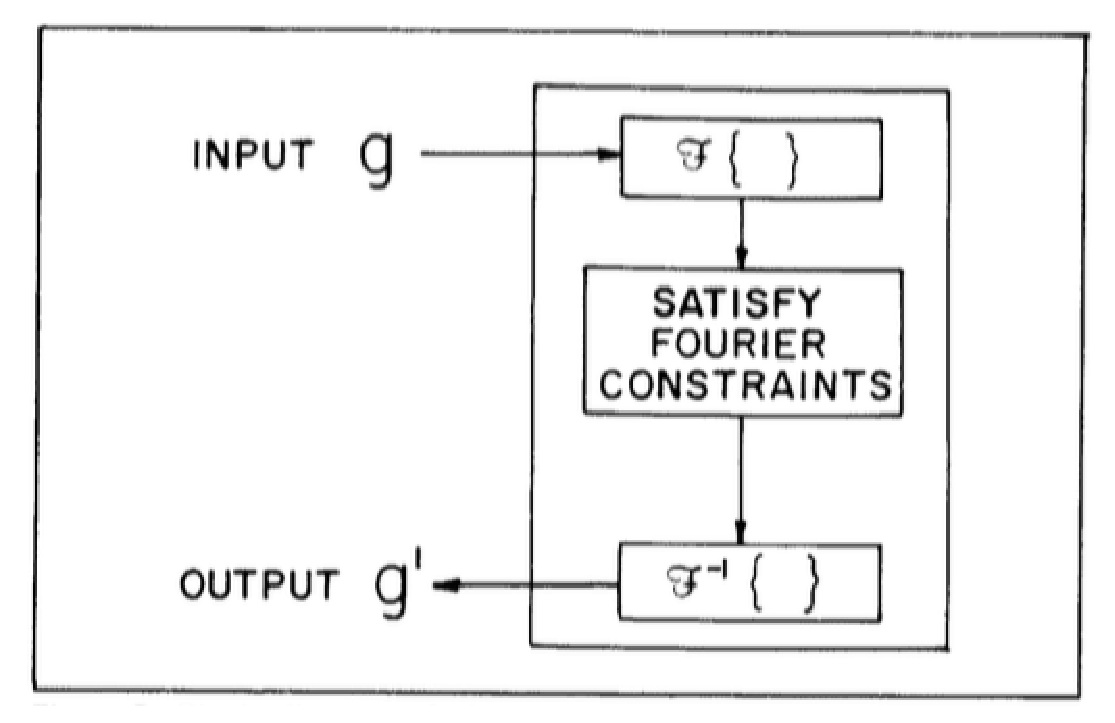
\includegraphics[height=4in]{figures/principle}
\end{tabular}
}
\caption{The principle of an input-output iterative Fourier transform algorithm.
The compared algorithms differ in the choice of input for subsequent iteration~\cite{Fienup:1980ge}.
}
\label{fig:principle}
\vspace{-4mm}
\end{figure}

The input-output algorithm we used, $g_{k+1}$, is with the following
updating process according to~\cite{Fienup:1980ge}:

%Equation
\begin{equation}
g_{k+1} = g_{k} + \Delta g(x) = g_{k} + \beta*\Delta g_d(x) 
\label{eq:IO}
\end{equation}

where $\Delta g_d(x) $ is defined as

\begin{equation}
\Delta g_d(x) = [|f(x)|*\frac{g'(x)}{|g'(x)|}-g'(x)]+[|f(x)|*\frac{g'(x)}{|g'(x)|}-|f(x)|*\frac{g(x)}{|g(x)|}]
\end{equation}

Output-output method has a different equation than Eq.~\ref{eq:IO}, instead of
modifying the input of the previous iteration, the output of the iteration,
$g'_k$ is used~\cite{Fienup3}:

\begin{equation}
g_{k+1} = g'_{k} + \Delta g(x)  
\label{eq:OO}
\end{equation}

In the simulations in the following chapters, we used $\beta = 1$ for IO
and OO implementations.
Another modification on IO is MIO~\cite{Chang:1994wt}, where $\beta$ from Eq.~\ref{eq:IO} is modified
with an exponentially damping term, $\alpha$, such that Eq.~\ref{eq:IO} becomes:

\begin{equation}
g_{k+1} = g_{k} + \Delta g(x) = g'_{k} + \frac{\beta}{\alpha^k}*\Delta g_d(x) 
\label{eq:OO}
\end{equation}

In our simulation for MIO, we chose $\beta = 1$ and $\alpha = 1.2$, Please note that
the performance of MIO can be optimized further by exploring the performance of the different
parameter pairs of $\beta$ and $\alpha$.

The last algorithm, HIO, differ in the sense that it apply different
updating rule for $g_{k+1}$ according to the spatial support. $g_{k+1} =  g'_{k}$ if
the updating area fall into the spatial support; $g_{k+1} =  g_{k} + \beta*\Delta g(x)$,
if the updating area is outside the spatial support~\cite{Fienup3} ($\beta$
is chosen to be 0.9 for the two HIO simulations).


\begin{figure}[t]
\centerline{
\begin{tabular}{c}
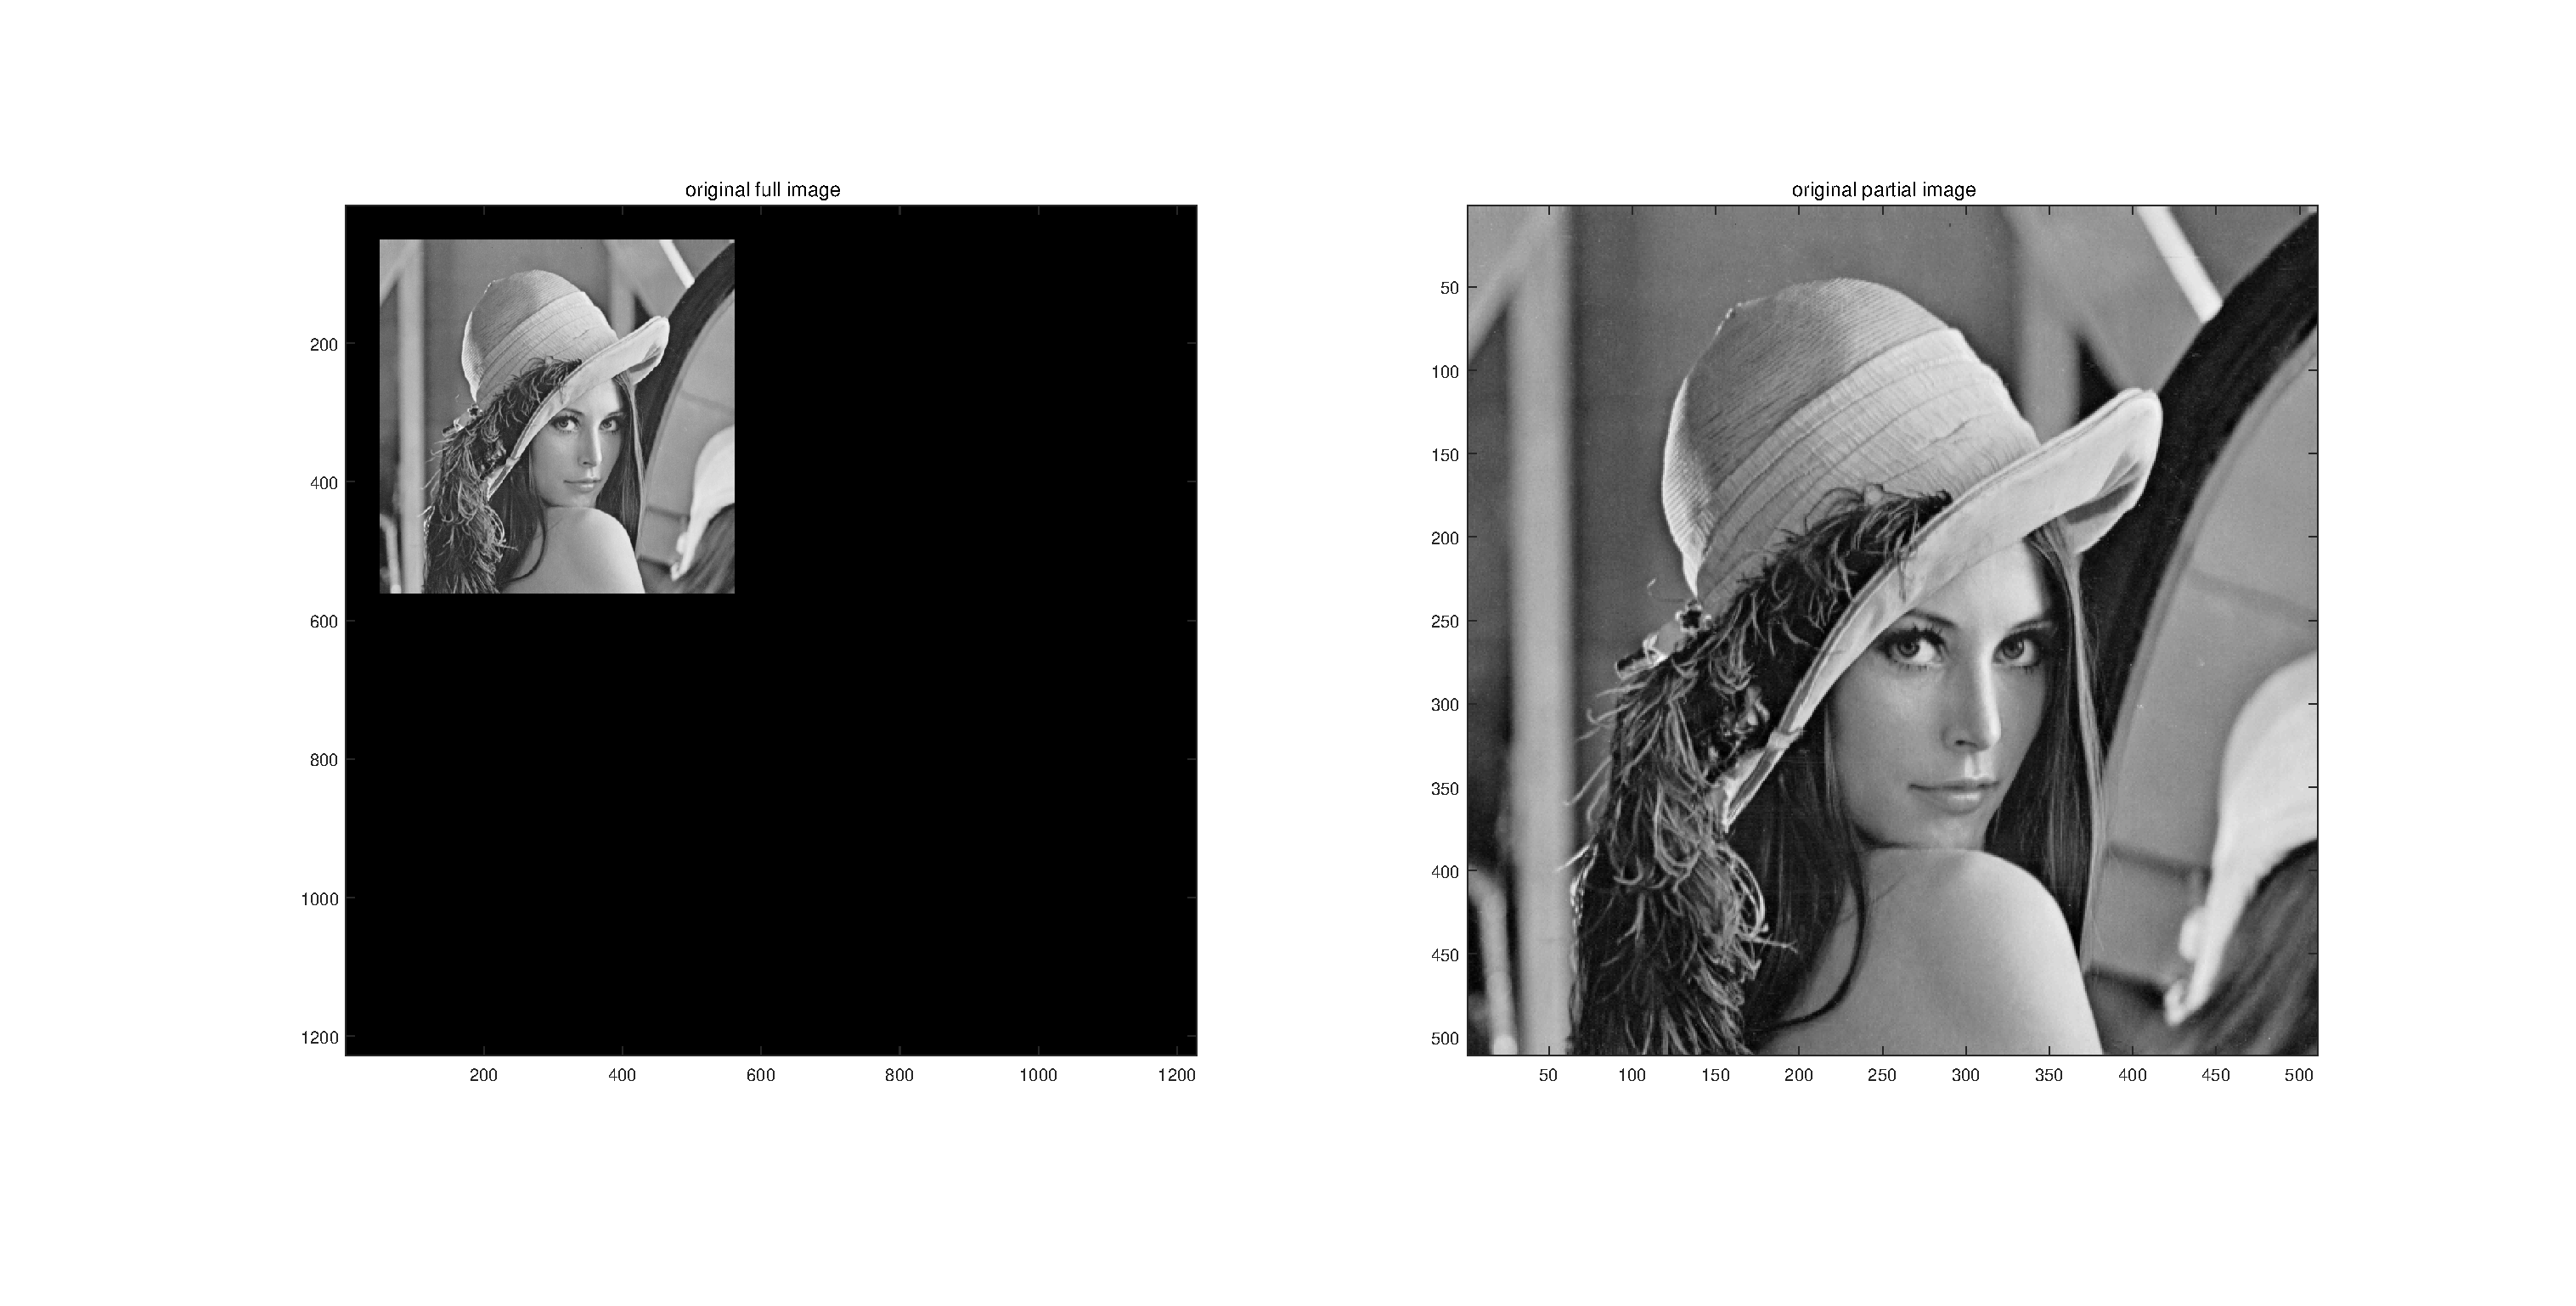
\includegraphics[height=3in]{figures/original}\\
\vspace{-2mm}
\end{tabular}
}
\caption{Original Lena image
}
\label{fig:original}
\end{figure}

\chapter{\Large Beam Shaping DOE}
\label{ch:compare}

The simulation for beam shaping DOE is defined as follows: we want to shape the 
illuminating plane wave incident on a DOE with quantized magnitude and quantized
phase, so that the produced complex diffraction pattern is the same as the 
desired complex image. We generate a complex large image with random phases at
each pixel as our desired image, the original magnitude of Lena image is placed in the 
first quadrant as shown in Fig.~\ref{fig:original}. 
Our goal is to design a DOE that is capable of generating this desired complex 
diffraction at far-field.
The DOE is designed to only has quantized magnitude and quantized
phase in the first quadrant to provide a spatial support.

The magnitude of the resulted DOEs and their corresponding magnitude of 
diffraction pattern are shown in Fig.~\ref{fig:50IO} for 50 IO iterations;
Fig.~\ref{fig:50OO} for 50 OO iterations; and Fig.~\ref{fig:50HIO} for 50 HIO
iterations, all with 256 magnitude quantization and 10 phase quantization.
Please note that the diagonal line is a result of latex image display, there
was no such line in MATLAB display.

\begin{figure}[t]
\centerline{
\begin{tabular}{c}
\includegraphics[height=3in]{figures/full_50IO_256_10}\\
\vspace{-2mm}
\end{tabular}
}
\caption{DOE and shaped diffraction pattern after 50 IO iterations.
}
\label{fig:50IO}
\end{figure}


\begin{figure}[t]
\centerline{
\begin{tabular}{c}
\includegraphics[height=3in]{figures/full_50OO_256_10}\\
\vspace{-2mm}
\end{tabular}
}
\caption{DOE and shaped diffraction pattern after 50 OO iterations.
}
\label{fig:50OO}
\end{figure}

\begin{figure}[t]
\centerline{
\begin{tabular}{c}
\includegraphics[height=3in]{figures/full_50HIO_256_10}\\
\vspace{-2mm}
\end{tabular}
}
\caption{DOE and shaped diffraction pattern after 50 HIO iterations.
}
\label{fig:50HIO}
\end{figure}

The magnitude of the resulted DOE and the corresponding magnitude of 
diffraction pattern for MIO algorithms are shown in \ref{fig:50MIO},
we also compare here the effect of using different number of 
levels of quantization. It clearly shows that more quantization lead
to a better result.

\begin{figure}[t]
\centerline{
\begin{tabular}{c}
\includegraphics[height=3in]{figures/full_50MIO_100_4}\\\
(a) 100 mangitude quantization and 4 phase quantization.\\
\includegraphics[height=3in]{figures/full_50MIO_256_10}\\
(b) 256 mangitude quantization and 10 phase quantization.\\
\end{tabular}
}
\caption{DOE and shaped diffraction pattern after 50 MIO iterations with
different quantization choices.
}
\label{fig:50MIO}
\vspace{-4mm}
\end{figure}

In Fig.~\ref{fig:DOEresidual}, we record the residual for the different
algorithms at each iteration to compare their performance. The residual
is defined as the ratio of the Euclidean norm of the difference between 
the diffraction pattern and goal image over the Euclidean norm of the
goal image. We can see that HIO is the best performing algorithm and MIO
is better than IO and OO after 20 iterations. We also notice that more
quantization levels allow more accurate representation, and more accurate
diffraction pattern generation.

\begin{figure}[t]
\centerline{
\begin{tabular}{c}
\includegraphics[height=8in]{figures/residualcompare}
\end{tabular}
}
\caption{The performance of algorithms with different quantization after
50 iterations.
}
\label{fig:DOEresidual}
\vspace{-4mm}
\end{figure}

\chapter{\Large Computer Generated Holography}
\label{ch:CGH}

Similarly, the algorithms can be used to generate holographic patterns
that will reconstruct the desired image after backpropagation.
The simulation for CGH is defined as follows: we want to design a holographic
pattern with quantized magnitude and quantized
phase, so that after backpropagation, the hologram will generate the
desired complex image. We generate a complex large image with random phases at
each pixel as our desired image, the original Lena image is placed in the 
first quadrant as shown in Fig.~\ref{fig:original}. The holograms have no 
special spatial support in this case so we compare IO, OO and MIO only.

The magnitude of the magnitude of the reconstructed images and 
the holograms that generated the images are shown in Fig.~\ref{fig:20IO} 
for 20 IO iterations; Fig.~\ref{fig:20OO} for 20 OO iterations; 
and Fig.~\ref{fig:20MIO} for 50 MIO iterations, 
all with 256 magnitude quantization and 10 phase quantization.
Please note again, that the diagonal line is a result of latex image display, 
there was no such line in MATLAB display.

\begin{figure}[t]
\centerline{
\begin{tabular}{c}
\includegraphics[height=3in]{figures/h_full_20IO_256_10}\\
\vspace{-2mm}
\end{tabular}
}
\caption{Reconstructed image and its hologram after 20 IO iterations.
}
\label{fig:20IO}
\end{figure}


\begin{figure}[t]
\centerline{
\begin{tabular}{c}
\includegraphics[height=3in]{figures/h_full_20OO_256_10}\\
\vspace{-2mm}
\end{tabular}
}
\caption{Reconstructed image and its hologram after 20 OO iterations.
}
\label{fig:20OO}
\end{figure}

\begin{figure}[t]
\centerline{
\begin{tabular}{c}
\includegraphics[height=3in]{figures/h_full_20MIO_256_10}\\
\vspace{-2mm}
\end{tabular}
}
\caption{Reconstructed image and its hologram after 20 MIO iterations.
}
\label{fig:20MIO}
\end{figure}

As we are comparing complex matrices, the showcased reconstructed
images in figures are not a good indicators because they are absolute valued.
We turn to comparing the residual convergence curve to determine which algorithm
is better.

In Fig.~\ref{fig:CGHresidual}, we record the residual for the different
algorithms at each iteration to compare their performance.
We can see that OO is the best performing algorithm and MIO
is performing better than IO. We also notice that more
quantization levels allow more accurate representation, and better
holographic quality.

\begin{figure}[t]
\centerline{
\begin{tabular}{c}
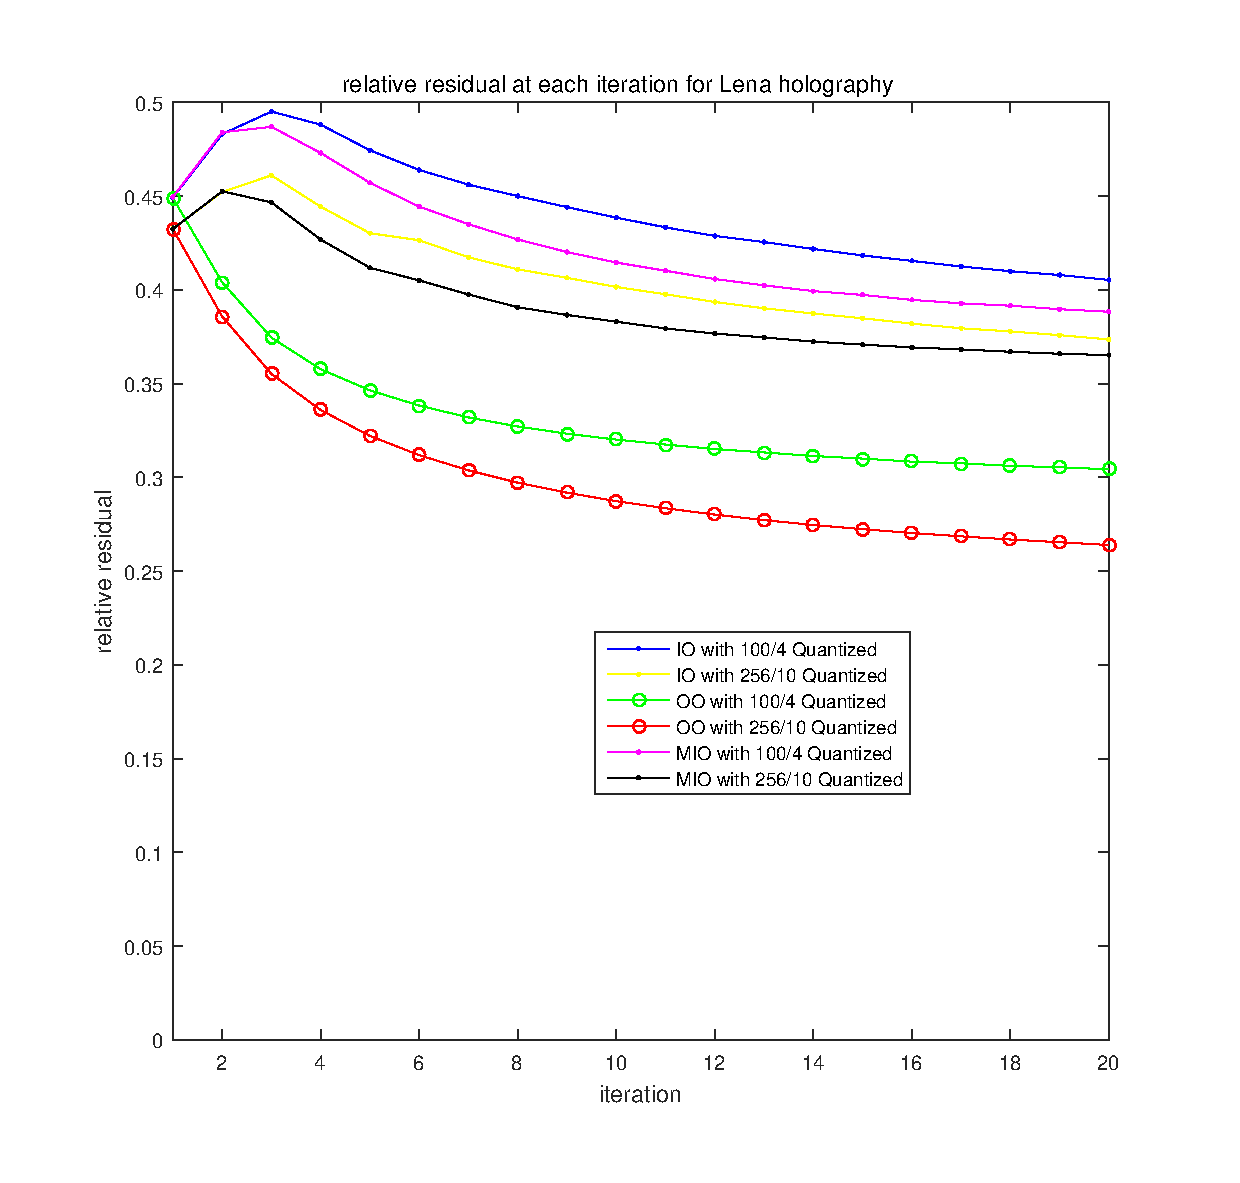
\includegraphics[height=8in]{figures/h_residualcompare}
\end{tabular}
}
\caption{The performance of algorithms with different quantization after
50 iterations.
}
\label{fig:CGHresidual}
\vspace{-4mm}
\end{figure}

\chapter{\Large Conclusion}
The performance of the tested iterative algorithms are showing
consistent characteristics in two different implementations: 
beam shaping DOE design and CGH design. Out of the compared algorithms,
the two variances of the basic IO: MIO, OO performs better than the basic IO.
MIO and HIO perform better in DOE design while OO performs better
in hologram generation.

\bibliography{reference}
\addcontentsline{toc}{chapter}{\bibname}
\begin{appendices}
\chapter{MATLAB Codes}
\label{ch:codes}
\singlespacing

Here, we attach report\_script\_beam\_shaper.m for the DOE
implementaion in Chap.~\ref{ch:compare} and report\_script\_image\_generation.m
for the CGH programming in Chap.~\ref{ch:CGH}.

The following is from report\_script\_beam\_shaper.m:


\begin{lstlisting} 
%% IO with 100/4
%% Preparations
clear;
close all;
%% parameters
itermax =50;
alpha = 1;
phasequantizer = 4;
magnitudequantizer = 100;

lena512 = imread('lena512.bmp');
X = im2double(lena512);
i = sqrt(-1);
Sample = 1.2;
loose = 0;
[imn1, imn2] = size(X);
imn11       = round(Sample * (imn1+2*loose));
% size of the image with zero paddings
imn22       = round(Sample * (imn2+2*loose));
image1   = zeros(imn11,imn22);   % image with zero paddings
start1   = round(1 + (imn11-imn1)/2);   % position of the true image
end1     = start1 + imn1 - 1;
start2   = round(1 + (imn22-imn2)/2);
end2     = start2 + imn2 - 1;
image1(start1:end2,start2:end2) = X;

%% build quadrant put into first quardrant
Sample = 2;
loose = 0;
[imn1, imn2] = size(image1);
imn11       = round(Sample * (imn1+2*loose));
% size of the image with zero paddings
imn22       = round(Sample * (imn2+2*loose));
image   = zeros(imn11,imn22);                 % image with zero paddings
image(start1:end2,start2:end2) = X;

imagetype = -2;
image     = image.*exp(i*unifrnd(0,2*pi,imn11,imn22));
% complex images have random phases in [0,2*pi]


S1start   = start1 - loose;
% In the case where the image has a loose support,
S1end     = end2   + loose;
% only a loose position of the true image is given
S2start   = start2 - loose;
S2end     = end2   + loose;

Index  = [imn1 , imn2 ; imn11 , imn22 ; S1start , S1end; S2start , S2end];
% data to input

X0  = generatestart(imagetype,Index);

%% IO  
N11          = Index(2,1); %size after zeropadding
N22          = Index(2,2); %size after zeropadding
N1start   = start1; %index where the true image start
N1end    = end2;
N2start  = start2;
N2end    = end2;

%% initiation
Xk           = X0;      % Xk
XkP          = X0;      % Pf{Xk}
iterres      = [];      % record residual at each iteration
iterchange   = [];      % record ||XkP{k}-XkP{k-1}||/||XkP{k-1}||

%% IO iteration
for iter = 1 : itermax  %iterate over IO
    TemMatrix = XkP;     % record XkP input from the previous iteration
    %% compute Pf{Xk}
    XkP   = Xk; %new input modified
    FXk  = fft2(XkP);
    FXkP = abs(image).*exp(i*angle(FXk)); %*(FXk./abs(FXk));
    XkP  = ifft2(FXkP); %new output
    %% calculate delta_g
    termA =  abs(ifft(image)).*(XkP./abs(XkP)); termA(isnan(termA)) = 0;
    termB =  abs(ifft(image)).*(Xk./abs(Xk)); termB(isnan(termB)) = 0;
    delta_g = termA -XkP+termA-termB;
    %% apply IO step
    new     = zeros(N11,N22);
    %% apply IO on zero paddings
%     new(:,1:N2start-1)              = Xk(:,1:N2start-1) + ...
%     alpha * delta_g(:,1:N2start-1);
%     new(:,N2end+1:N22)              = Xk(:,N2end+1:N22) + ...
%     alpha * delta_g(:,N2end+1:N22);
%     new(1:N1start-1,N2start:N2end)  = Xk(1:N1start-1,N2start:N2end)...
%     + alpha * delta_g(1:N1start-1,N2start:N2end);
%     new(N1end+1:N11,N2start:N2end)  = Xk(N1end+1:N11,N2start:N2end)...
%     + alpha * delta_g(N1end+1:N11,N2start:N2end);
    %% apply IO in support
if imagetype == -2
    new(N1start:N1end,N2start:N2end) = Xk(N1start:N1end,N2start:N2end)...
        + alpha * delta_g(N1start:N1end,N2start:N2end);
    newabs= floor(magnitudequantizer*abs(new)./(max(max(abs(new)))))...
        ./magnitudequantizer*max(max(abs(new)));
    newangle = floor(phasequantizer*angle(new)./(2*pi))...
        ./phasequantizer*2*pi;
    new_quant= newabs.*exp(i.*newangle);
    Xk             = new_quant;
end
%     new = Xk + + alpha * delta_g;
%     newabs= floor(magnitudequantizer*abs(new)./(max(max(abs(new)))))...
%         ./magnitudequantizer*max(max(abs(new)));
%     newangle = floor(phasequantizer*angle(new)./(2*pi))...
%         ./phasequantizer*2*pi;
%     new_quant= newabs.*exp(i.*newangle);
%     Xk             = new_quant;

    %% record residual
    Xtem = zeros(N11,N22);
    Xtem(N1start:N1end,N2start:N2end) = ...
        projection(XkP(N1start:N1end,N2start:N2end),imagetype);
    intensityerr = norm(abs(fft2(Xtem))-abs(image),'fro')^2;
    intensityerr = sqrt(intensityerr) / sqrt(norm(abs(image),'fro')^2);
    iterres(iter)  = intensityerr;
    %% record the change of XkP
    iterchange(iter) = norm(TemMatrix-XkP,'fro')/norm(TemMatrix,'fro');
    %% display data
    fprintf('%6.0f residual = %6.4f p change = %6.6f p \n',iter,...
        100*intensityerr,100*iterchange(iter))
end

Xrec   = Xk;

hologram = fft2(Xrec);
%% plot the magnitudes of the recovered image
figure(1)
subplot(1,2,1)
imagesc(abs(Xrec(start1:end1,start2:end2)));
axis equal
axis([1 end1-start1 1 end2-start2])
colormap(gray)
title(['DOE with ' num2str(magnitudequantizer)...
    ' discrete magnitude and ' num2str(phasequantizer) ' discrete phase'])
subplot(1,2,2)
imagesc(abs(hologram(start1:end1,start2:end2)))
axis equal
axis([1 end1-start1 1 end2-start2])
colormap(gray)
title('magnitude of produced beam pattern') 
savefig('partial_50IO_100_4.fig')

figure(2)
subplot(1,2,1)
imagesc(abs(Xrec));
axis equal
axis([1 imn11 1 imn22])
colormap(gray)
title(['DOE with ' num2str(magnitudequantizer)...
    ' discrete magnitude and ' num2str(phasequantizer) ' discrete phase'])
subplot(1,2,2)
imagesc(abs(hologram))
axis equal
axis([1 imn11 1 imn22])
colormap(gray)
title('magnitude of produced beam pattern')
savefig('full_50IO_100_4.fig')

iterres_100_4_IO = iterres;
save('50IO_100_4_residue.mat','iterres_100_4_IO')

%% IO First with 256/10
clear;
close all;
%% parameters
itermax =50;
alpha = 1;
phasequantizer = 10;
magnitudequantizer = 256;

lena512 = imread('lena512.bmp');
X = im2double(lena512);
i = sqrt(-1);
Sample = 1.2;
loose = 0;
[imn1, imn2] = size(X);
imn11       = round(Sample * (imn1+2*loose));
% size of the image with zero paddings
imn22       = round(Sample * (imn2+2*loose));
image1   = zeros(imn11,imn22);           % image with zero paddings
start1   = round(1 + (imn11-imn1)/2);    % position of the true image
end1     = start1 + imn1 - 1;
start2   = round(1 + (imn22-imn2)/2);
end2     = start2 + imn2 - 1;
image1(start1:end2,start2:end2) = X;

%% build quadrant put into first quardrant
Sample = 2;
loose = 0;
[imn1, imn2] = size(image1);
imn11       = round(Sample * (imn1+2*loose));
% size of the image with zero paddings
imn22       = round(Sample * (imn2+2*loose));
image   = zeros(imn11,imn22);          % image with zero paddings
image(start1:end2,start2:end2) = X;

imagetype = -2;
image     = image.*exp(i*unifrnd(0,2*pi,imn11,imn22));
% complex images have random phases in [0,2*pi]


S1start   = start1 - loose;
% In the case where the image has a loose support,
S1end     = end2   + loose;
% only a loose position of the true image is given
S2start   = start2 - loose;
S2end     = end2   + loose;

Index  = [imn1 , imn2 ; imn11 , imn22 ; S1start , S1end; S2start , S2end];
% data to input

X0  = generatestart(imagetype,Index);

%% IO  
N11          = Index(2,1); %size after zeropadding
N22          = Index(2,2); %size after zeropadding
N1start   = start1; %index where the true image start
N1end    = end2;
N2start  = start2;
N2end    = end2;

%% initiation
Xk           = X0;      % Xk
XkP          = X0;      % Pf{Xk}
iterres      = [];      % record residual at each iteration
iterchange   = [];      % record ||XkP{k}-XkP{k-1}||/||XkP{k-1}||

%% IO iteration
for iter = 1 : itermax  %iterate over IO
    TemMatrix = XkP;     % record XkP input from the previous iteration
    %% compute Pf{Xk}
    XkP   = Xk; %new input modified
    FXk  = fft2(XkP);
    FXkP = abs(image).*exp(i*angle(FXk)); %*(FXk./abs(FXk));
    XkP  = ifft2(FXkP); %new output
    %% calculate delta_g
    termA =  abs(ifft(image)).*(XkP./abs(XkP)); termA(isnan(termA)) = 0;
    termB =  abs(ifft(image)).*(Xk./abs(Xk)); termB(isnan(termB)) = 0;
    delta_g = termA -XkP+termA-termB;
    %% apply IO step
    new     = zeros(N11,N22);
    %% apply IO on zero paddings
%     new(:,1:N2start-1)              = Xk(:,1:N2start-1) + ...
%         alpha * delta_g(:,1:N2start-1);
%     new(:,N2end+1:N22)              = Xk(:,N2end+1:N22) + ...
%         alpha * delta_g(:,N2end+1:N22);
%     new(1:N1start-1,N2start:N2end)  = Xk(1:N1start-1,N2start:N2end)...
%         + alpha * delta_g(1:N1start-1,N2start:N2end);
%     new(N1end+1:N11,N2start:N2end)  = Xk(N1end+1:N11,N2start:N2end)...
%         + alpha * delta_g(N1end+1:N11,N2start:N2end);
%% apply IO in support
if imagetype == -2
    new(N1start:N1end,N2start:N2end) = Xk(N1start:N1end,N2start:N2end)...
        + alpha * delta_g(N1start:N1end,N2start:N2end);
    newabs= floor(magnitudequantizer*abs(new)./(max(max(abs(new)))))...
        ./magnitudequantizer*max(max(abs(new)));
    newangle = floor(phasequantizer*angle(new)./(2*pi))...
        ./phasequantizer*2*pi;
    new_quant= newabs.*exp(i.*newangle);
    Xk             = new_quant;
end
    %% record residual
    Xtem = zeros(N11,N22);
    Xtem(N1start:N1end,N2start:N2end) = ...
        projection(XkP(N1start:N1end,N2start:N2end),imagetype);
    intensityerr = norm(abs(fft2(Xtem))-abs(image),'fro')^2;
    intensityerr = sqrt(intensityerr) / sqrt(norm(abs(image),'fro')^2);
    iterres(iter)  = intensityerr;
    %% record the change of XkP
    iterchange(iter) = norm(TemMatrix-XkP,'fro')/norm(TemMatrix,'fro');
    %% display data
    fprintf('%6.0f residual = %6.4f p change = %6.6f p \n',iter,...
        100*intensityerr,100*iterchange(iter))
end

Xrec   = Xk;

hologram = fft2(Xrec);
%% plot the magnitudes of the recovered image
figure(1)
subplot(1,2,1)
imagesc(abs(Xrec(start1:end1,start2:end2)));
axis equal
axis([1 end1-start1 1 end2-start2])
colormap(gray)
title(['DOE with ' num2str(magnitudequantizer)...
    ' discrete magnitude and ' num2str(phasequantizer) ' discrete phase'])
subplot(1,2,2)
imagesc(abs(hologram(start1:end1,start2:end2)))
axis equal
axis([1 end1-start1 1 end2-start2])
colormap(gray)
title('magnitude of produced beam pattern')
savefig('partial_50IO_256_10.fig')

figure(2)
subplot(1,2,1)
imagesc(abs(Xrec));
axis equal
axis([1 imn11 1 imn22])
colormap(gray)
title(['DOE with ' num2str(magnitudequantizer)...
    ' discrete magnitude and ' num2str(phasequantizer) ' discrete phase'])
subplot(1,2,2)
imagesc(abs(hologram))
axis equal
axis([1 imn11 1 imn22])
colormap(gray)
title('magnitude of produced beam pattern') 
savefig('full_50IO_256_10.fig')

iterres_256_10_IO = iterres;
save('50IO_256_10_residue.mat','iterres_256_10_IO')

%% MIO with 100/4

%% Preparations
clear;
close all;
%% parameters
itermax =50;
alpha = 1;
beta = 1.2;
phasequantizer = 4;
magnitudequantizer = 100;

lena512 = imread('lena512.bmp');
X = im2double(lena512);

i = sqrt(-1);
Sample = 1.2;
loose = 0;
[imn1, imn2] = size(X);
imn11       = round(Sample * (imn1+2*loose)); 
% size of the image with zero paddings
imn22       = round(Sample * (imn2+2*loose));
image1   = zeros(imn11,imn22);                 % image with zero paddings
start1   = round(1 + (imn11-imn1)/2);          % position of the true image
end1     = start1 + imn1 - 1;
start2   = round(1 + (imn22-imn2)/2);
end2     = start2 + imn2 - 1;
image1(start1:end2,start2:end2) = X;

%% build quadrant put into first quardrant
Sample = 2;
loose = 0;
[imn1, imn2] = size(image1);
imn11       = round(Sample * (imn1+2*loose));
% size of the image with zero paddings
imn22       = round(Sample * (imn2+2*loose));
image   = zeros(imn11,imn22);                 % image with zero paddings
image(start1:end2,start2:end2) = X;

imagetype = -2;
image     = image.*exp(i*unifrnd(0,2*pi,imn11,imn22));
% complex images have random phases in [0,2*pi]


S1start   = start1 - loose;
% In the case where the image has a loose support,
S1end     = end2   + loose;
% only a loose position of the true image is given
S2start   = start2 - loose;
S2end     = end2   + loose;

Index  = [imn1 , imn2 ; imn11 , imn22 ; S1start , S1end; S2start , S2end];
% data to input

X0  = generatestart(imagetype,Index);

%% MIO  
N11          = Index(2,1); %size after zeropadding
N22          = Index(2,2); %size after zeropadding
N1start   = start1; %index where the true image start
N1end    = end2;
N2start  = start2;
N2end    = end2;

%% initiation
Xk           = X0;      % Xk
XkP          = X0;      % Pf{Xk}
iterres      = [];      % record residual at each iteration
iterchange   = [];      % record ||XkP{k}-XkP{k-1}||/||XkP{k-1}||

%% MIO iteration
for iter = 1 : itermax  %iterate over MIO
    TemMatrix = XkP;     % record XkP from the previous iteration
    %% compute Pf{Xk}
    XkP   = Xk;
    FXk  = fft2(XkP);
    FXkP = abs(image).*exp(i*angle(FXk)); %*(FXk./abs(FXk));
    XkP  = ifft2(FXkP);
    %% calculate delta_g
    termA =  abs(ifft(image)).*(XkP./abs(XkP)); termA(isnan(termA)) = 0;
    termB =  abs(ifft(image)).*(Xk./abs(Xk)); termB(isnan(termB)) = 0;
    delta_g = termA -XkP+termA-termB;
    %% apply MIO step
    new     = zeros(N11,N22);
%     %% apply MIO on zero paddings
%     new(:,1:N2start-1)              = Xk(:,1:N2start-1) +...
%         alpha/beta^(iter-1) * delta_g(:,1:N2start-1);
%     new(:,N2end+1:N22)              = Xk(:,N2end+1:N22) +...
%         alpha/beta^(iter-1) * delta_g(:,N2end+1:N22);
%     new(1:N1start-1,N2start:N2end)  = Xk(1:N1start-1,N2start:N2end) +...
%         alpha/beta^(iter-1) * delta_g(1:N1start-1,N2start:N2end);
%     new(N1end+1:N11,N2start:N2end)  = Xk(N1end+1:N11,N2start:N2end) +...
%         alpha/beta^(iter-1) * delta_g(N1end+1:N11,N2start:N2end);
%% apply MIO in support
if imagetype == -2
new(N1start:N1end,N2start:N2end) = ...
    Xk(N1start:N1end,N2start:N2end) + alpha/beta^(iter-1) * ...
    delta_g(N1start:N1end,N2start:N2end);
newabs= floor(magnitudequantizer*abs(new)./(max(max(abs(new)))))...
    ./magnitudequantizer*max(max(abs(new)));
newangle = floor(phasequantizer*angle(new)./(2*pi))./phasequantizer*2*pi;
new_quant= newabs.*exp(i.*newangle);
Xk             = new_quant;
end
    %% record residual
    Xtem = zeros(N11,N22);
    Xtem(N1start:N1end,N2start:N2end) = projection(XkP(N1start:N1end,...
        N2start:N2end),imagetype);
    intensityerr = norm(abs(fft2(Xtem))-abs(image),'fro')^2;
    intensityerr = sqrt(intensityerr) / sqrt(norm(abs(image),'fro')^2);
    iterres(iter)  = intensityerr;
    %% record the change of XkP
    iterchange(iter) = norm(TemMatrix-XkP,'fro')/norm(TemMatrix,'fro');
    %% display data
    fprintf('%6.0f residual = %6.4f p change = %6.6f p \n',...
        iter,100*intensityerr,100*iterchange(iter))
end

Xrec   = Xk;

hologram = fft2(Xrec);
%% plot the magnitudes of the recovered image
figure(1)
subplot(1,2,1)
imagesc(abs(Xrec(start1:end1,start2:end2)));
axis equal
axis([1 end1-start1 1 end2-start2])
colormap(gray)
title(['DOE with ' num2str(magnitudequantizer)...
    ' discrete magnitude and ' num2str(phasequantizer) ' discrete phase'])
subplot(1,2,2)
imagesc(abs(hologram(start1:end1,start2:end2)))
axis equal
axis([1 end1-start1 1 end2-start2])
colormap(gray)
title('magnitude of produced beam pattern') 
savefig('partial_50MIO_100_4.fig')

figure(2)
subplot(1,2,1)
imagesc(abs(Xrec));
axis equal
axis([1 imn11 1 imn22])
colormap(gray)
title(['DOE with ' num2str(magnitudequantizer)...
    ' discrete magnitude and ' num2str(phasequantizer) ' discrete phase'])
subplot(1,2,2)
imagesc(abs(hologram))
axis equal
axis([1 imn11 1 imn22])
colormap(gray)
title('magnitude of produced beam pattern') 
savefig('full_50MIO_100_4.fig')

iterres_100_4_MIO = iterres;
save('50MIO_100_4_residue.mat','iterres_100_4_MIO')

%% MIO with256/10

%% Preparations
clear;
close all;
%% parameters
itermax =50;
alpha = 1;
beta = 1.2;
phasequantizer = 10;
magnitudequantizer = 256;

lena512 = imread('lena512.bmp');
X = im2double(lena512);
i = sqrt(-1);
Sample = 1.2;
loose = 0;
[imn1, imn2] = size(X);
imn11       = round(Sample * (imn1+2*loose));  
% size of the image with zero paddings
imn22       = round(Sample * (imn2+2*loose));
image1   = zeros(imn11,imn22);                 % image with zero paddings
start1   = round(1 + (imn11-imn1)/2);          % position of the true image
end1     = start1 + imn1 - 1;
start2   = round(1 + (imn22-imn2)/2);
end2     = start2 + imn2 - 1;
image1(start1:end2,start2:end2) = X;

%% build quadrant put into first quardrant
Sample = 2;
loose = 0;
[imn1, imn2] = size(image1);
imn11       = round(Sample * (imn1+2*loose));
% size of the image with zero paddings
imn22       = round(Sample * (imn2+2*loose));
image   = zeros(imn11,imn22);                 % image with zero paddings
image(start1:end2,start2:end2) = X;

imagetype = -2;
image     = image.*exp(i*unifrnd(0,2*pi,imn11,imn22));
% complex images have random phases in [0,2*pi]


S1start   = start1 - loose;
% In the case where the image has a loose support,
S1end     = end2   + loose;
% only a loose position of the true image is given
S2start   = start2 - loose;
S2end     = end2   + loose;

Index  = [imn1 , imn2 ; imn11 , imn22 ; S1start , S1end; S2start , S2end];
% data to input

X0  = generatestart(imagetype,Index);

%% MIO  
N11          = Index(2,1); %size after zeropadding
N22          = Index(2,2); %size after zeropadding
N1start   = start1; %index where the true image start
N1end    = end2;
N2start  = start2;
N2end    = end2;

%% initiation
Xk           = X0;      % Xk
XkP          = X0;      % Pf{Xk}
iterres      = [];      % record residual at each iteration
iterchange   = [];      % record ||XkP{k}-XkP{k-1}||/||XkP{k-1}||

%% MIO iteration
for iter = 1 : itermax  %iterate over MIO
    TemMatrix = XkP;     % record XkP from the previous iteration
    %% compute Pf{Xk}
    XkP   = Xk;
    FXk  = fft2(XkP);
    FXkP = abs(image).*exp(i*angle(FXk)); %*(FXk./abs(FXk));
    XkP  = ifft2(FXkP);
    %% calculate delta_g
    termA =  abs(ifft(image)).*(XkP./abs(XkP)); termA(isnan(termA)) = 0;
    termB =  abs(ifft(image)).*(Xk./abs(Xk)); termB(isnan(termB)) = 0;
    delta_g = termA -XkP+termA-termB;
    %% apply MIO step
    new     = zeros(N11,N22);
%     %% apply MIO on zero paddings
%     new(:,1:N2start-1)              = Xk(:,1:N2start-1) +...
%         alpha/beta^(iter-1) * delta_g(:,1:N2start-1);
%     new(:,N2end+1:N22)              = Xk(:,N2end+1:N22) +...
%         alpha/beta^(iter-1) * delta_g(:,N2end+1:N22);
%     new(1:N1start-1,N2start:N2end)  = Xk(1:N1start-1,N2start:N2end) +...
%         alpha/beta^(iter-1) * delta_g(1:N1start-1,N2start:N2end);
%     new(N1end+1:N11,N2start:N2end)  = Xk(N1end+1:N11,N2start:N2end) +...
%         alpha/beta^(iter-1) * delta_g(N1end+1:N11,N2start:N2end);
%     %% apply MIO in support
if imagetype == -2
new(N1start:N1end,N2start:N2end) = ...
    Xk(N1start:N1end,N2start:N2end) + alpha/beta^(iter-1) * ...
    delta_g(N1start:N1end,N2start:N2end);
newabs= floor(magnitudequantizer*abs(new)./(max(max(abs(new)))))...
    ./magnitudequantizer*max(max(abs(new)));
newangle = floor(phasequantizer*angle(new)./(2*pi))./phasequantizer*2*pi;
new_quant= newabs.*exp(i.*newangle);
Xk             = new_quant;
end
    %% record residual
    Xtem = zeros(N11,N22);
    Xtem(N1start:N1end,N2start:N2end) = projection(...
        XkP(N1start:N1end,N2start:N2end),imagetype);
    intensityerr = norm(abs(fft2(Xtem))-abs(image),'fro')^2;
    intensityerr = sqrt(intensityerr) / sqrt(norm(abs(image),'fro')^2);
    iterres(iter)  = intensityerr;
    %% record the change of XkP
    iterchange(iter) = norm(TemMatrix-XkP,'fro')/norm(TemMatrix,'fro');
    %% display data
    fprintf('%6.0f residual = %6.4f p change = %6.6f p \n',...
        iter,100*intensityerr,100*iterchange(iter))
end

Xrec   = Xk;

hologram = fft2(Xrec);

%% plot the magnitudes of the recovered image
figure(1)
subplot(1,2,1)
imagesc(abs(Xrec(start1:end1,start2:end2)));
axis equal
axis([1 end1-start1 1 end2-start2])
colormap(gray)
title(['DOE with ' num2str(magnitudequantizer)...
    ' discrete magnitude and ' num2str(phasequantizer) ' discrete phase'])
subplot(1,2,2)
imagesc(abs(hologram(start1:end1,start2:end2)))
axis equal
axis([1 end1-start1 1 end2-start2])
colormap(gray)
title('magnitude of produced beam pattern') 
savefig('partial_50MIO_256_10.fig')
    
figure(2)
subplot(1,2,1)
imagesc(abs(Xrec));
axis equal
axis([1 imn11 1 imn22])
colormap(gray)
title(['DOE with ' num2str(magnitudequantizer)...
    ' discrete magnitude and ' num2str(phasequantizer) ' discrete phase'])
subplot(1,2,2)
imagesc(abs(hologram))
axis equal
axis([1 imn11 1 imn22])
colormap(gray)
title('magnitude of produced beam pattern') 
savefig('full_50MIO_256_10.fig')

iterres_256_10_MIO = iterres;
save('50MIO_256_10_residue.mat','iterres_256_10_MIO')

%% HIO with 100/4
%% Preparations
clear;
close all;
%% parameters
itermax =50;

beta = 0.8;
phasequantizer = 4;
magnitudequantizer = 100;

lena512 = imread('lena512.bmp');
X = im2double(lena512);


i = sqrt(-1);
Sample = 1.2;
loose = 0;
[imn1, imn2] = size(X);
imn11       = round(Sample * (imn1+2*loose));
% size of the image with zero paddings
imn22       = round(Sample * (imn2+2*loose));
image1   = zeros(imn11,imn22);                 % image with zero paddings
start1   = round(1 + (imn11-imn1)/2);          % position of the true image
end1     = start1 + imn1 - 1;
start2   = round(1 + (imn22-imn2)/2);
end2     = start2 + imn2 - 1;
image1(start1:end2,start2:end2) = X;

%% build quadrant put into first quardrant
Sample = 2;
loose = 0;
[imn1, imn2] = size(image1);
imn11       = round(Sample * (imn1+2*loose));
% size of the image with zero paddings
imn22       = round(Sample * (imn2+2*loose));
image   = zeros(imn11,imn22);                 % image with zero paddings
image(start1:end2,start2:end2) = X;

imagetype = -2;
image     = image.*exp(i*unifrnd(0,2*pi,imn11,imn22));
% complex images have random phases in [0,2*pi]


S1start   = start1 - loose;
% In the case where the image has a loose support,
S1end     = end2   + loose;
% only a loose position of the true image is given
S2start   = start2 - loose;
S2end     = end2   + loose;

Index  = [imn1 , imn2 ; imn11 , imn22 ; S1start , S1end; S2start , S2end];
% data to input

X0  = generatestart(imagetype,Index);

%% HIO  
N11          = Index(2,1); %size after zeropadding
N22          = Index(2,2); %size after zeropadding
N1start   = start1; %index where the true image start
N1end    = end2;
N2start  = start2;
N2end    = end2;

%% initiation
Xk           = X0;      % Xk
XkP          = X0;      % Pf{Xk}
iterres      = [];      % record residual at each iteration
iterchange   = [];      % record ||XkP{k}-XkP{k-1}||/||XkP{k-1}||


%% HIO iteration
for iter = 1 : itermax  %iterate over HIO
    TemMatrix = XkP;     % record XkP from the previous iteration
    %% compute Pf{Xk}
    XkP   = Xk;
    FXk  = fft2(XkP);
    FXkP = abs(image).*exp(i*angle(FXk)); %*(FXk./abs(FXk));
    XkP  = ifft2(FXkP);
    
    %% apply HIO step
    new     = zeros(N11,N22);
    %% apply HIO on zero paddings
    new(:,1:N2start-1)              = Xk(:,1:N2start-1) -...
        beta * XkP(:,1:N2start-1);
    new(:,N2end+1:N22)              = Xk(:,N2end+1:N22) - ...
        beta * XkP(:,N2end+1:N22);
    new(1:N1start-1,N2start:N2end)  = ...
        Xk(1:N1start-1,N2start:N2end) - ...
        beta * XkP(1:N1start-1,N2start:N2end);
    new(N1end+1:N11,N2start:N2end)  = ...
        Xk(N1end+1:N11,N2start:N2end) - ...
        beta * XkP(N1end+1:N11,N2start:N2end);
    %% apply HIO in support
    if imagetype == -2
        new(N1start:N1end,N2start:N2end) = ...
            XkP(N1start:N1end,N2start:N2end);
        newabs= floor(magnitudequantizer*...
            abs(new)./(max(max(abs(new)))))./...
            magnitudequantizer*max(max(abs(new)));
        newangle = floor(phasequantizer*...
            angle(new)./(2*pi))./phasequantizer*2*pi;
        new_quant= newabs.*exp(i.*newangle);
        Xk             = new_quant;
    end
    %% record residual
    Xtem = zeros(N11,N22);
    Xtem(N1start:N1end,N2start:N2end) = ...
        projection(XkP(N1start:N1end,N2start:N2end),imagetype);
    intensityerr = norm(abs(fft2(Xtem))-abs(image),'fro')^2;
    intensityerr = sqrt(intensityerr) / sqrt(norm(abs(image),'fro')^2);
    iterres(iter)  = intensityerr;
    %% record the change of XkP
    iterchange(iter) = norm(TemMatrix-XkP,'fro')/norm(TemMatrix,'fro');
    %% display data
    fprintf('%6.0f residual = %6.4f p change = %6.6f p \n',...
        iter,100*intensityerr,100*iterchange(iter))
    
end

Xrec   = Xk;

hologram = fft2(Xrec);
%% plot the magnitudes of the recovered image
figure(1)
subplot(1,2,1)
imagesc(abs(Xrec(start1:end1,start2:end2)));
axis equal
axis([1 end1-start1 1 end2-start2])
colormap(gray)
title(['DOE with ' num2str(magnitudequantizer)...
    ' discrete magnitude and ' num2str(phasequantizer) ' discrete phase'])
subplot(1,2,2)
imagesc(abs(hologram(start1:end1,start2:end2)))
axis equal
axis([1 end1-start1 1 end2-start2])
colormap(gray)
title('magnitude of produced beam pattern') 
savefig('partial_50HIO_100_4.fig')

figure(2)
subplot(1,2,1)
imagesc(abs(Xrec));
axis equal
axis([1 imn11 1 imn22])
colormap(gray)
title(['DOE with ' num2str(magnitudequantizer)...
    ' discrete magnitude and ' num2str(phasequantizer) ' discrete phase'])
subplot(1,2,2)
imagesc(abs(hologram))
axis equal
axis([1 imn11 1 imn22])
colormap(gray)
title('magnitude of produced beam pattern') 
savefig('full_50HIO_100_4.fig')

iterres_100_4_HIO = iterres;
save('50HIO_100_4_residue.mat','iterres_100_4_HIO')

%% HIO with 256/10
%% Preparations
clear;
close all;
%% parameters
itermax =50;
ifer = 0;
beta = 0.9;
phasequantizer = 10;
magnitudequantizer = 256;

lena512 = imread('lena512.bmp');
X = im2double(lena512);
i = sqrt(-1);
Sample = 1.2;
loose = 0;
[imn1, imn2] = size(X);
imn11       = round(Sample * (imn1+2*loose));  
% size of the image with zero paddings
imn22       = round(Sample * (imn2+2*loose));
image1   = zeros(imn11,imn22);                 % image with zero paddings
start1   = round(1 + (imn11-imn1)/2);          % position of the true image
end1     = start1 + imn1 - 1;
start2   = round(1 + (imn22-imn2)/2);
end2     = start2 + imn2 - 1;
image1(start1:end2,start2:end2) = X;

%% build quadrant put into first quardrant
Sample = 2;
loose = 0;
[imn1, imn2] = size(image1);
imn11       = round(Sample * (imn1+2*loose));
% size of the image with zero paddings
imn22       = round(Sample * (imn2+2*loose));
image   = zeros(imn11,imn22);          % image with zero paddings
image(start1:end2,start2:end2) = X;

imagetype = -2;
image     = image.*exp(i*unifrnd(0,2*pi,imn11,imn22));
% complex images have random phases in [0,2*pi]


S1start   = start1 - loose;
% In the case where the image has a loose support,
S1end     = end2   + loose;
% only a loose position of the true image is given
S2start   = start2 - loose;
S2end     = end2   + loose;

Index  = [imn1 , imn2 ; imn11 , imn22 ; S1start , S1end; S2start , S2end];
% data to input

X0  = generatestart(imagetype,Index);

%% HIO  
N11          = Index(2,1); %size after zeropadding
N22          = Index(2,2); %size after zeropadding
N1start   = start1; %index where the true image start
N1end    = end2;
N2start  = start2;
N2end    = end2;
N1        = N1end - N1start + 1; %number of real data points 1D
N2        = N2end - N2start + 1;
P           = 1;


%% initiation
Xk           = X0;      % Xk
XkP          = X0;      % Pf{Xk}
iterres      = [];      % record residual at each iteration
iterchange   = [];      % record ||XkP{k}-XkP{k-1}||/||XkP{k-1}||
Y           = X0;
Y_abs_fro   = norm(Y,'fro')^2;
Y_abs       = abs(Y);              % Fourier intensity data
Y_abs_fro   = sqrt(Y_abs_fro);     % Euclidean norm

%% HIO iteration
for iter = 1 : itermax  %iterate over HIO
    TemMatrix = XkP;     % record XkP from the previous iteration
    %% compute Pf{Xk}
    XkP   = Xk;
    FXk  = fft2(XkP);
    FXkP = abs(image).*exp(i*angle(FXk)); %*(FXk./abs(FXk));
    XkP  = ifft2(FXkP);
    
    %% apply HIO step
    new     = zeros(N11,N22);
    %% apply HIO on zero paddings
    new(:,1:N2start-1)              = Xk(:,1:N2start-1) -...
        beta * XkP(:,1:N2start-1);
    new(:,N2end+1:N22)              = Xk(:,N2end+1:N22) - ...
        beta * XkP(:,N2end+1:N22);
    new(1:N1start-1,N2start:N2end)  = ...
        Xk(1:N1start-1,N2start:N2end) - ...
        beta * XkP(1:N1start-1,N2start:N2end);
    new(N1end+1:N11,N2start:N2end)  = ...
        Xk(N1end+1:N11,N2start:N2end) - ...
        beta * XkP(N1end+1:N11,N2start:N2end);
    %% apply HIO in support
    if imagetype == -2
        new(N1start:N1end,N2start:N2end) = ...
            XkP(N1start:N1end,N2start:N2end);
        newabs= floor(magnitudequantizer*...
            abs(new)./(max(max(abs(new)))))./...
            magnitudequantizer*max(max(abs(new)));
        newangle = floor(phasequantizer*...
            angle(new)./(2*pi))./phasequantizer*2*pi;
        new_quant= newabs.*exp(i.*newangle);
        Xk             = new_quant;
    end
    %% record residual
    Xtem = zeros(N11,N22);
    Xtem(N1start:N1end,N2start:N2end) = ...
        projection(XkP(N1start:N1end,N2start:N2end),imagetype);
    intensityerr = norm(abs(fft2(Xtem))-abs(image),'fro')^2;
    intensityerr = sqrt(intensityerr) / sqrt(norm(abs(image),'fro')^2);
    iterres(iter)  = intensityerr;
    %% record the change of XkP
    iterchange(iter) = norm(TemMatrix-XkP,'fro')/norm(TemMatrix,'fro');
    %% display data
    fprintf('%6.0f residual = %6.4f p change = %6.6f p \n',...
        iter,100*intensityerr,100*iterchange(iter))
end

hiostep  = length(iterres);

Xrec   = Xk;

hologram = fft2(Xrec);
%% plot the magnitudes of the recovered image
figure(1)
subplot(1,2,1)
imagesc(abs(Xrec(start1:end1,start2:end2)));
axis equal
axis([1 end1-start1 1 end2-start2])
colormap(gray)
title(['DOE with ' num2str(magnitudequantizer)...
    ' discrete magnitude and ' num2str(phasequantizer) ' discrete phase'])
subplot(1,2,2)
imagesc(abs(hologram(start1:end1,start2:end2)))
axis equal
axis([1 end1-start1 1 end2-start2])
colormap(gray)
title('magnitude of produced beam pattern') 
savefig('partial_50HIO_256_10.fig')
figure(2)
subplot(1,2,1)
imagesc(abs(Xrec));
axis equal
axis([1 imn11 1 imn22])
colormap(gray)
title(['DOE with ' num2str(magnitudequantizer)...
    ' discrete magnitude and ' num2str(phasequantizer) ' discrete phase'])
subplot(1,2,2)
imagesc(abs(hologram))
axis equal
axis([1 imn11 1 imn22])
colormap(gray)
title('magnitude of produced beam pattern') 
savefig('full_50HIO_256_10.fig')

iterres_256_10_HIO = iterres;
save('50HIO_256_10_residue.mat','iterres_256_10_HIO')

%% OO with 100/4
%% Preparations
clear;
close all;
%% parameters
itermax =50;
alpha = 1;
phasequantizer = 4;
magnitudequantizer = 100;

lena512 = imread('lena512.bmp');
X = im2double(lena512);
i = sqrt(-1);
Sample = 1.2;
loose = 0;
[imn1, imn2] = size(X);
imn11       = round(Sample * (imn1+2*loose));
% size of the image with zero paddings
imn22       = round(Sample * (imn2+2*loose));
image1   = zeros(imn11,imn22);   % image with zero paddings
start1   = round(1 + (imn11-imn1)/2);   % position of the true image
end1     = start1 + imn1 - 1;
start2   = round(1 + (imn22-imn2)/2);
end2     = start2 + imn2 - 1;
image1(start1:end2,start2:end2) = X;

%% build quadrant put into first quardrant
Sample = 2;
loose = 0;
[imn1, imn2] = size(image1);
imn11       = round(Sample * (imn1+2*loose));
% size of the image with zero paddings
imn22       = round(Sample * (imn2+2*loose));
image   = zeros(imn11,imn22);                 % image with zero paddings
image(start1:end2,start2:end2) = X;

imagetype = -2;
image     = image.*exp(i*unifrnd(0,2*pi,imn11,imn22));
% complex images have random phases in [0,2*pi]


S1start   = start1 - loose;
% In the case where the image has a loose support,
S1end     = end2   + loose;
% only a loose position of the true image is given
S2start   = start2 - loose;
S2end     = end2   + loose;

Index  = [imn1 , imn2 ; imn11 , imn22 ; S1start , S1end; S2start , S2end];
% data to input

X0  = generatestart(imagetype,Index);

%% OO
N11          = Index(2,1); %size after zeropadding
N22          = Index(2,2); %size after zeropadding
N1start   = start1; %index where the true image start
N1end    = end2;
N2start  = start2;
N2end    = end2;

%% initiation
Xk           = X0;      % Xk
XkP          = X0;      % Pf{Xk}
iterres      = [];      % record residual at each iteration
iterchange   = [];      % record ||XkP{k}-XkP{k-1}||/||XkP{k-1}||

%% OO iteration
for iter = 1 : itermax  %iterate over IO
    TemMatrix = XkP;     % record XkP input from the previous iteration
    %% compute Pf{Xk}
    XkP   = Xk; %new input modified
    FXk  = fft2(XkP);
    FXkP = abs(image).*exp(i*angle(FXk)); %*(FXk./abs(FXk));
    XkP  = ifft2(FXkP); %new output
    %% calculate delta_g
    termA =  abs(ifft(image)).*(XkP./abs(XkP)); termA(isnan(termA)) = 0;
    termB =  abs(ifft(image)).*(Xk./abs(Xk)); termB(isnan(termB)) = 0;
    delta_g = termA -XkP+termA-termB;
    %% apply IO step
    new     = zeros(N11,N22);
    %% apply IO on zero paddings
    %     new(:,1:N2start-1)              = Xk(:,1:N2start-1) + ...
    %     alpha * delta_g(:,1:N2start-1);
    %     new(:,N2end+1:N22)              = Xk(:,N2end+1:N22) + ...
    %     alpha * delta_g(:,N2end+1:N22);
    %     new(1:N1start-1,N2start:N2end)  = Xk(1:N1start-1,N2start:N2end)...
    %     + alpha * delta_g(1:N1start-1,N2start:N2end);
    %     new(N1end+1:N11,N2start:N2end)  = Xk(N1end+1:N11,N2start:N2end)...
    %     + alpha * delta_g(N1end+1:N11,N2start:N2end);
    %% apply IO in support
if imagetype == -2
    new(N1start:N1end,N2start:N2end) = XkP(N1start:N1end,N2start:N2end)...
        + alpha * delta_g(N1start:N1end,N2start:N2end);
    newabs= floor(magnitudequantizer*abs(new)./(max(max(abs(new)))))...
        ./magnitudequantizer*max(max(abs(new)));
    newangle = floor(phasequantizer*angle(new)./(2*pi))...
        ./phasequantizer*2*pi;
    new_quant= newabs.*exp(i.*newangle);
    Xk             = new_quant;
end
%     new = Xk + + alpha * delta_g;
%     newabs= floor(magnitudequantizer*abs(new)./(max(max(abs(new)))))...
%         ./magnitudequantizer*max(max(abs(new)));
%     newangle = floor(phasequantizer*angle(new)./(2*pi))...
%         ./phasequantizer*2*pi;
%     new_quant= newabs.*exp(i.*newangle);
%     Xk             = new_quant;
    
    %% record residual
    Xtem = zeros(N11,N22);
    Xtem(N1start:N1end,N2start:N2end) = ...
        projection(XkP(N1start:N1end,N2start:N2end),imagetype);
    intensityerr = norm(abs(fft2(Xtem))-abs(image),'fro')^2;
    intensityerr = sqrt(intensityerr) / sqrt(norm(abs(image),'fro')^2);
    iterres(iter)  = intensityerr;
    %% record the change of XkP
    iterchange(iter) = norm(TemMatrix-XkP,'fro')/norm(TemMatrix,'fro');
    %% display data
    fprintf('%6.0f residual = %6.4f p change = %6.6f p \n',iter,...
        100*intensityerr,100*iterchange(iter))
end

Xrec   = Xk;

hologram = fft2(Xrec);
%% plot the magnitudes of the recovered image
figure(1)
subplot(1,2,1)
imagesc(abs(Xrec(start1:end1,start2:end2)));
axis equal
axis([1 end1-start1 1 end2-start2])
colormap(gray)
title(['DOE with ' num2str(magnitudequantizer)...
    ' discrete magnitude and ' num2str(phasequantizer) ' discrete phase'])
subplot(1,2,2)
imagesc(abs(hologram(start1:end1,start2:end2)))
axis equal
axis([1 end1-start1 1 end2-start2])
colormap(gray)
title('magnitude of produced beam pattern') 
savefig('partial_50OO_100_4.fig')

figure(2)
subplot(1,2,1)
imagesc(abs(Xrec));
axis equal
axis([1 imn11 1 imn22])
colormap(gray)
title(['DOE with ' num2str(magnitudequantizer)...
    ' discrete magnitude and ' num2str(phasequantizer) ' discrete phase'])
subplot(1,2,2)
imagesc(abs(hologram))
axis equal
axis([1 imn11 1 imn22])
colormap(gray)
title('magnitude of produced beam pattern') 
savefig('full_50OO_100_4.fig')

iterres_100_4_OO = iterres;
save('50OO_100_4_residue.mat','iterres_100_4_OO')

%% OO with 256/10
%% Preparations
clear;
close all;
%% parameters
itermax =50;
alpha = 1;
phasequantizer = 10;
magnitudequantizer = 256;

lena512 = imread('lena512.bmp');
X = im2double(lena512);
i = sqrt(-1);
Sample = 1.2;
loose = 0;
[imn1, imn2] = size(X);
imn11       = round(Sample * (imn1+2*loose));
% size of the image with zero paddings
imn22       = round(Sample * (imn2+2*loose));
image1   = zeros(imn11,imn22);   % image with zero paddings
start1   = round(1 + (imn11-imn1)/2);   % position of the true image
end1     = start1 + imn1 - 1;
start2   = round(1 + (imn22-imn2)/2);
end2     = start2 + imn2 - 1;
image1(start1:end2,start2:end2) = X;

%% build quadrant put into first quardrant
Sample = 2;
loose = 0;
[imn1, imn2] = size(image1);
imn11       = round(Sample * (imn1+2*loose));
% size of the image with zero paddings
imn22       = round(Sample * (imn2+2*loose));
image   = zeros(imn11,imn22);                 % image with zero paddings
image(start1:end2,start2:end2) = X;

imagetype = -2;
image     = image.*exp(i*unifrnd(0,2*pi,imn11,imn22));
% complex images have random phases in [0,2*pi]


S1start   = start1 - loose;
% In the case where the image has a loose support,
S1end     = end2   + loose;
% only a loose position of the true image is given
S2start   = start2 - loose;
S2end     = end2   + loose;

Index  = [imn1 , imn2 ; imn11 , imn22 ; S1start , S1end; S2start , S2end];
% data to input

X0  = generatestart(imagetype,Index);

%% OO
N11          = Index(2,1); %size after zeropadding
N22          = Index(2,2); %size after zeropadding
N1start   = start1; %index where the true image start
N1end    = end2;
N2start  = start2;
N2end    = end2;

%% initiation
Xk           = X0;      % Xk
XkP          = X0;      % Pf{Xk}
iterres      = [];      % record residual at each iteration
iterchange   = [];      % record ||XkP{k}-XkP{k-1}||/||XkP{k-1}||

%% OO iteration
for iter = 1 : itermax  %iterate over IO
    TemMatrix = XkP;     % record XkP input from the previous iteration
    %% compute Pf{Xk}
    XkP   = Xk; %new input modified
    FXk  = fft2(XkP);
    FXkP = abs(image).*exp(i*angle(FXk)); %*(FXk./abs(FXk));
    XkP  = ifft2(FXkP); %new output
    %% calculate delta_g
    termA =  abs(ifft(image)).*(XkP./abs(XkP)); termA(isnan(termA)) = 0;
    termB =  abs(ifft(image)).*(Xk./abs(Xk)); termB(isnan(termB)) = 0;
    delta_g = termA -XkP+termA-termB;
    %% apply IO step
    new     = zeros(N11,N22);
%% apply IO on zero paddings
%     new(:,1:N2start-1)              = Xk(:,1:N2start-1) + ...
%     alpha * delta_g(:,1:N2start-1);
%     new(:,N2end+1:N22)              = Xk(:,N2end+1:N22) + ...
%     alpha * delta_g(:,N2end+1:N22);
%     new(1:N1start-1,N2start:N2end)  = Xk(1:N1start-1,N2start:N2end)...
%     + alpha * delta_g(1:N1start-1,N2start:N2end);
%     new(N1end+1:N11,N2start:N2end)  = Xk(N1end+1:N11,N2start:N2end)...
%     + alpha * delta_g(N1end+1:N11,N2start:N2end);
    %% apply IO in support
if imagetype == -2
    new(N1start:N1end,N2start:N2end) = XkP(N1start:N1end,N2start:N2end)...
        + alpha * delta_g(N1start:N1end,N2start:N2end);
    newabs= floor(magnitudequantizer*abs(new)./(max(max(abs(new)))))...
        ./magnitudequantizer*max(max(abs(new)));
    newangle = floor(phasequantizer*angle(new)./(2*pi))...
        ./phasequantizer*2*pi;
    new_quant= newabs.*exp(i.*newangle);
    Xk             = new_quant;
end
%     new = Xk + + alpha * delta_g;
%     newabs= floor(magnitudequantizer*abs(new)./(max(max(abs(new)))))...
%         ./magnitudequantizer*max(max(abs(new)));
%     newangle = floor(phasequantizer*angle(new)./(2*pi))...
%         ./phasequantizer*2*pi;
%     new_quant= newabs.*exp(i.*newangle);
%     Xk             = new_quant;
    
    %% record residual
    Xtem = zeros(N11,N22);
    Xtem(N1start:N1end,N2start:N2end) = ...
        projection(XkP(N1start:N1end,N2start:N2end),imagetype);
    intensityerr = norm(abs(fft2(Xtem))-abs(image),'fro')^2;
    intensityerr = sqrt(intensityerr) / sqrt(norm(abs(image),'fro')^2);
    iterres(iter)  = intensityerr;
    %% record the change of XkP
    iterchange(iter) = norm(TemMatrix-XkP,'fro')/norm(TemMatrix,'fro');
    %% display data
    fprintf('%6.0f residual = %6.4f p change = %6.6f p \n',iter,...
        100*intensityerr,100*iterchange(iter))
end

Xrec   = Xk;

hologram = fft2(Xrec);
%% plot the magnitudes of the recovered image
figure(1)
subplot(1,2,1)
imagesc(abs(Xrec(start1:end1,start2:end2)));
axis equal
axis([1 end1-start1 1 end2-start2])
colormap(gray)
title(['DOE with ' num2str(magnitudequantizer)...
    ' discrete magnitude and ' num2str(phasequantizer) ' discrete phase'])
subplot(1,2,2)
imagesc(abs(hologram(start1:end1,start2:end2)))
axis equal
axis([1 end1-start1 1 end2-start2])
colormap(gray)
title('magnitude of produced beam pattern') 
savefig('partial_50OO_256_10.fig')

figure(2)
subplot(1,2,1)
imagesc(abs(Xrec));
axis equal
axis([1 imn11 1 imn22])
colormap(gray)
title(['DOE with ' num2str(magnitudequantizer)...
    ' discrete magnitude and ' num2str(phasequantizer) ' discrete phase'])
subplot(1,2,2)
imagesc(abs(hologram))
axis equal
axis([1 imn11 1 imn22])
colormap(gray)
title('magnitude of produced beam pattern') 
savefig('full_50OO_256_10.fig')

iterres_256_10_OO = iterres;
save('50OO_256_10_residue.mat','iterres_256_10_OO')

figure(3)
subplot(1,2,1)
imagesc(abs(image));
axis equal
axis([1 imn11 1 imn22])
colormap(gray)
title('original full image')
subplot(1,2,2)
imagesc(abs(image(start1:end1,start2:end2)));
axis equal
axis([1 end1-start1 1 end2-start2])
colormap(gray)
title('original partial image')
savefig('original.fig')

load('50HIO_100_4_residue.mat')
load('50HIO_256_10_residue.mat')
load('50IO_100_4_residue.mat')
load('50IO_256_10_residue.mat')
load('50OO_100_4_residue.mat')
load('50OO_256_10_residue.mat')
load('50MIO_100_4_residue.mat')
load('50MIO_256_10_residue.mat')

figure(4)
plot(1:length(iterres_100_4_IO),iterres_100_4_IO,'.-b',...
    1:length(iterres_256_10_IO),iterres_256_10_IO,'.-y',...
    1:length(iterres_100_4_OO),iterres_100_4_OO,'-og',...
    1:length(iterres_256_10_OO),iterres_256_10_OO,'-or',...
    1:length(iterres_100_4_MIO),iterres_100_4_MIO,'.-m',...
    1:length(iterres_256_10_MIO),iterres_256_10_MIO,'.-k',...
    1:length(iterres_100_4_HIO),iterres_100_4_HIO,'.-r',...
    1:length(iterres_256_10_HIO),iterres_256_10_HIO,'.-g');
axis([1 length(iterres_100_4_IO) 0 0.5])
legend('IO with 100/4 Quantized','IO with 256/10 Quantized',...
    'OO with 100/4 Quantized','OO with 256/10 Quantized',...
    'MIO with 100/4 Quantized','MIO with 256/10 Quantized',...
    'HIO with 100/4 Quantized','HIO with 256/10 Quantized');
title('relative residual at each iteration for DOE shaping Lena')
xlabel('iteration')
ylabel('relative residual')
savefig('residualcompare.fig')
\end{lstlisting}

The following is code from the file named report\_script\_image\_generation.m:

\begin{lstlisting} 
%% IO with 100/4
%% Preparations
clear;
close all;
%% parameters
itermax = 20;
alpha = 1;
phasequantizer = 4;
magnitudequantizer = 100;

lena512 = imread('lena512.bmp');
X = im2double(lena512);
i = sqrt(-1);
Sample = 1.2;
loose = 0;
[imn1, imn2] = size(X);
imn11       = round(Sample * (imn1+2*loose));
% size of the image with zero paddings
imn22       = round(Sample * (imn2+2*loose));
image1   = zeros(imn11,imn22);   % image with zero paddings
start1   = round(1 + (imn11-imn1)/2);   % position of the true image
end1     = start1 + imn1 - 1;
start2   = round(1 + (imn22-imn2)/2);
end2     = start2 + imn2 - 1;
image1(start1:end2,start2:end2) = X;

%% build quadrant put into first quardrant
Sample = 2;
loose = 0;
[imn1, imn2] = size(image1);
imn11       = round(Sample * (imn1+2*loose));
% size of the image with zero paddings
imn22       = round(Sample * (imn2+2*loose));
image   = zeros(imn11,imn22);                 % image with zero paddings
image(start1:end2,start2:end2) = X;

imagetype = -2;
image     = image.*exp(i*unifrnd(0,2*pi,imn11,imn22));
% complex images have random phases in [0,2*pi]


S1start   = start1 - loose;% In the case where the image has a loose support,
S1end     = end2   + loose;% only a loose position of the true image is given
S2start   = start2 - loose;
S2end     = end2   + loose;

Index  = [imn1 , imn2 ; imn11 , imn22 ; S1start , S1end; S2start , S2end];
% data to input

X0  = generatestart(imagetype,Index);

%% IO  
N11          = Index(2,1); %size after zeropadding
N22          = Index(2,2); %size after zeropadding
N1start   = start1; %index where the true image start
N1end    = end2;
N2start  = start2;
N2end    = end2;

%% initiation
Xk           = X0;      % Xk
XkP          = X0;      % Pf{Xk}
iterres      = [];      % record residual at each iteration
iterchange   = [];      % record ||XkP{k}-XkP{k-1}||/||XkP{k-1}||

Y_abs = abs(fft2(image));

%% IO iteration
for iter = 1 : itermax  %iterate over IO
    TemMatrix = XkP;     % record XkP input from the previous iteration
    %% compute Pf{Xk}
    XkP   = Xk; %new input modified
    FXk  = fft2(XkP);
    FXkP = Y_abs.*exp(i*angle(FXk)); %*(FXk./abs(FXk));
    FXkP_abs= floor(magnitudequantizer*abs(FXkP)./(max(max(abs(FXkP)))))...
      ./magnitudequantizer*max(max(abs(FXkP)));
    FXkP_angle = floor(phasequantizer*angle(FXkP)./(2*pi))...
      ./phasequantizer*2*pi;
    FXkP_quant= FXkP_abs.*exp(i.*FXkP_angle);
    XkP  = ifft2(FXkP_quant); %new output
    %% calculate delta_g
    termA =  abs(image).*(XkP./abs(XkP)); termA(isnan(termA)) = 0;
    termB =  abs(image).*(XkP./abs(XkP)); termB(isnan(termA)) = 0;
    delta_g = termA -XkP+termA-termB;
    %% apply IO step
    new     = zeros(N11,N22);
    %% apply IO on zero paddings
    new(:,1:N2start-1)              = Xk(:,1:N2start-1) + ...
    alpha * delta_g(:,1:N2start-1);
    new(:,N2end+1:N22)              = Xk(:,N2end+1:N22) + ...
    alpha * delta_g(:,N2end+1:N22);
    new(1:N1start-1,N2start:N2end)  = Xk(1:N1start-1,N2start:N2end)...
    + alpha * delta_g(1:N1start-1,N2start:N2end);
    new(N1end+1:N11,N2start:N2end)  = Xk(N1end+1:N11,N2start:N2end)...
    + alpha * delta_g(N1end+1:N11,N2start:N2end);
    %% apply IO in support
    if imagetype == -2
        new(N1start:N1end,N2start:N2end) = ...
            Xk(N1start:N1end,N2start:N2end)+ ...
            alpha * delta_g(N1start:N1end,N2start:N2end);
        Xk             = new;
    end
    %% record residual
    Xtem = zeros(N11,N22);
    Xtem(N1start:N1end,N2start:N2end) = ...
    projection(XkP(N1start:N1end,N2start:N2end),imagetype);
    intensityerr = norm(abs(fft2(Xtem))-Y_abs,'fro')^2;
    intensityerr = sqrt(intensityerr)/norm(Y_abs,'fro');
    iterres(iter)  = intensityerr;
    %% record the change of XkP
    iterchange(iter) = norm(TemMatrix-XkP,'fro')/norm(TemMatrix,'fro');
    %% display data
    fprintf('%6.0f residual = %6.4f p change = %6.6f p \n',iter,...
        100*intensityerr,100*iterchange(iter))
    Xrec   = XkP;
    figure(1)
    subplot(1,2,1)
    imagesc(abs(Xrec(start1:end1,start2:end2)));
    axis equal
    axis([1 end1-start1 1 end2-start2])
    colormap(gray)
    title('Hologram reconstructed image')
    subplot(1,2,2)
    imagesc(abs(FXkP_quant))
    axis equal
    axis([1 end1-start1 1 end2-start2])
    colormap(gray)
    title('Hologram')
    drawnow;
end



%% plot the magnitudes of the recovered image

figure(2)
subplot(1,2,1)
imagesc(abs(Xrec));
axis equal
axis([1 imn11 1 imn22])
colormap(gray)
title('Hologram reconstructed image')
subplot(1,2,2)
imagesc(abs(FXkP_quant))
axis equal
axis([1 imn11 1 imn22])
colormap(gray)
title(['Hologram with ' num2str(magnitudequantizer)...
    ' discrete magnitude and ' num2str(phasequantizer) ' discrete phase'])
savefig(['h_full_' num2str(itermax) 'IO_'... 
    num2str(magnitudequantizer) '_' num2str(phasequantizer) '.fig'])

iterres_100_4_IO = iterres;
save(['h_' num2str(itermax) 'IO_' num2str(magnitudequantizer)...
    '_' num2str(phasequantizer) '_residue.mat'],'iterres_100_4_IO')

%% IO First with 256/10
%% Preparations
clear;
close all;
%% parameters
itermax = 20;
alpha = 1;
phasequantizer = 10;
magnitudequantizer = 256;

lena512 = imread('lena512.bmp');
X = im2double(lena512);
i = sqrt(-1);
Sample = 1.2;
loose = 0;
[imn1, imn2] = size(X);
imn11       = round(Sample * (imn1+2*loose));
% size of the image with zero paddings
imn22       = round(Sample * (imn2+2*loose));
image1   = zeros(imn11,imn22);   % image with zero paddings
start1   = round(1 + (imn11-imn1)/2);   % position of the true image
end1     = start1 + imn1 - 1;
start2   = round(1 + (imn22-imn2)/2);
end2     = start2 + imn2 - 1;
image1(start1:end2,start2:end2) = X;

%% build quadrant put into first quardrant
Sample = 2;
loose = 0;
[imn1, imn2] = size(image1);
imn11       = round(Sample * (imn1+2*loose));
% size of the image with zero paddings
imn22       = round(Sample * (imn2+2*loose));
image   = zeros(imn11,imn22);                 % image with zero paddings
image(start1:end2,start2:end2) = X;

imagetype = -2;
image     = image.*exp(i*unifrnd(0,2*pi,imn11,imn22));
% complex images have random phases in [0,2*pi]


S1start   = start1 - loose;% In the case where the image has a loose support,
S1end     = end2   + loose;% only a loose position of the true image is given
S2start   = start2 - loose;
S2end     = end2   + loose;

Index  = [imn1 , imn2 ; imn11 , imn22 ; S1start , S1end; S2start , S2end];
% data to input

X0  = generatestart(imagetype,Index);

%% IO  
N11          = Index(2,1); %size after zeropadding
N22          = Index(2,2); %size after zeropadding
N1start   = start1; %index where the true image start
N1end    = end2;
N2start  = start2;
N2end    = end2;

%% initiation
Xk           = X0;      % Xk
XkP          = X0;      % Pf{Xk}
iterres      = [];      % record residual at each iteration
iterchange   = [];      % record ||XkP{k}-XkP{k-1}||/||XkP{k-1}||

Y_abs = abs(fft2(image));

%% IO iteration
for iter = 1 : itermax  %iterate over IO
    TemMatrix = XkP;     % record XkP input from the previous iteration
    %% compute Pf{Xk}
    XkP   = Xk; %new input modified
    FXk  = fft2(XkP);
    FXkP = Y_abs.*exp(i*angle(FXk)); %*(FXk./abs(FXk));
    FXkP_abs= floor(magnitudequantizer*abs(FXkP)./(max(max(abs(FXkP)))))...
      ./magnitudequantizer*max(max(abs(FXkP)));
    FXkP_angle = floor(phasequantizer*angle(FXkP)./(2*pi))...
      ./phasequantizer*2*pi;
    FXkP_quant= FXkP_abs.*exp(i.*FXkP_angle);
    XkP  = ifft2(FXkP_quant); %new output
    %% calculate delta_g
    termA =  abs(image).*(XkP./abs(XkP)); termA(isnan(termA)) = 0;
    termB =  abs(image).*(XkP./abs(XkP)); termB(isnan(termA)) = 0;
    delta_g = termA -XkP+termA-termB;
    %% apply IO step
    new     = zeros(N11,N22);
    %% apply IO on zero paddings
    new(:,1:N2start-1)              = Xk(:,1:N2start-1) + ...
    alpha * delta_g(:,1:N2start-1);
    new(:,N2end+1:N22)              = Xk(:,N2end+1:N22) + ...
    alpha * delta_g(:,N2end+1:N22);
    new(1:N1start-1,N2start:N2end)  = Xk(1:N1start-1,N2start:N2end)...
    + alpha * delta_g(1:N1start-1,N2start:N2end);
    new(N1end+1:N11,N2start:N2end)  = Xk(N1end+1:N11,N2start:N2end)...
    + alpha * delta_g(N1end+1:N11,N2start:N2end);
    %% apply IO in support
    if imagetype == -2
        new(N1start:N1end,N2start:N2end) = ...
            Xk(N1start:N1end,N2start:N2end)+ ...
            alpha * delta_g(N1start:N1end,N2start:N2end);
        Xk             = new;
    end
    %% record residual
    Xtem = zeros(N11,N22);
    Xtem(N1start:N1end,N2start:N2end) = ...
    projection(XkP(N1start:N1end,N2start:N2end),imagetype);
    intensityerr = norm(abs(fft2(Xtem))-Y_abs,'fro')^2;
    intensityerr = sqrt(intensityerr)/norm(Y_abs,'fro');
    iterres(iter)  = intensityerr;
    %% record the change of XkP
    iterchange(iter) = norm(TemMatrix-XkP,'fro')/norm(TemMatrix,'fro');
    %% display data
    fprintf('%6.0f residual = %6.4f p change = %6.6f p \n',iter,...
    100*intensityerr,100*iterchange(iter))
    Xrec   = XkP;
    figure(1)
    subplot(1,2,1)
    imagesc(abs(Xrec(start1:end1,start2:end2)));
    axis equal
    axis([1 end1-start1 1 end2-start2])
    colormap(gray)
    title('Hologram reconstructed image')
    subplot(1,2,2)
    imagesc(abs(FXkP_quant))
    axis equal
    axis([1 end1-start1 1 end2-start2])
    colormap(gray)
    title('Hologram')
    drawnow;
end

%% plot the magnitudes of the recovered image

figure(2)
subplot(1,2,1)
imagesc(abs(Xrec));
axis equal
axis([1 imn11 1 imn22])
colormap(gray)
title('Hologram reconstructed image')
subplot(1,2,2)
imagesc(abs(FXkP_quant))
axis equal
axis([1 imn11 1 imn22])
colormap(gray)
title(['Hologram with ' num2str(magnitudequantizer)...
    ' discrete magnitude and ' num2str(phasequantizer) ' discrete phase'])
savefig(['h_full_' num2str(itermax) 'IO_'... 
    num2str(magnitudequantizer) '_' num2str(phasequantizer) '.fig'])

iterres_256_10_IO = iterres;
save(['h_' num2str(itermax) 'IO_' num2str(magnitudequantizer)...
    '_' num2str(phasequantizer) '_residue.mat'],'iterres_256_10_IO')

%% OO with 100/4
%% Preparations
clear;
close all;
%% parameters
itermax = 20;
alpha = 1;
phasequantizer = 4;
magnitudequantizer = 100;

lena512 = imread('lena512.bmp');
X = im2double(lena512);
i = sqrt(-1);
Sample = 1.2;
loose = 0;
[imn1, imn2] = size(X);
imn11       = round(Sample * (imn1+2*loose));
% size of the image with zero paddings
imn22       = round(Sample * (imn2+2*loose));
image1   = zeros(imn11,imn22);   % image with zero paddings
start1   = round(1 + (imn11-imn1)/2);   % position of the true image
end1     = start1 + imn1 - 1;
start2   = round(1 + (imn22-imn2)/2);
end2     = start2 + imn2 - 1;
image1(start1:end2,start2:end2) = X;

%% build quadrant put into first quardrant
Sample = 2;
loose = 0;
[imn1, imn2] = size(image1);
imn11       = round(Sample * (imn1+2*loose));
% size of the image with zero paddings
imn22       = round(Sample * (imn2+2*loose));
image   = zeros(imn11,imn22);                 % image with zero paddings
image(start1:end2,start2:end2) = X;

imagetype = -2;
image     = image.*exp(i*unifrnd(0,2*pi,imn11,imn22));
% complex images have random phases in [0,2*pi]


S1start   = start1 - loose;% In the case where the image has a loose support,
S1end     = end2   + loose;% only a loose position of the true image is given
S2start   = start2 - loose;
S2end     = end2   + loose;

Index  = [imn1 , imn2 ; imn11 , imn22 ; S1start , S1end; S2start , S2end];
% data to input

X0  = generatestart(imagetype,Index);

%% OO  
N11          = Index(2,1); %size after zeropadding
N22          = Index(2,2); %size after zeropadding
N1start   = start1; %index where the true image start
N1end    = end2;
N2start  = start2;
N2end    = end2;

%% initiation
Xk           = X0;      % Xk
XkP          = X0;      % Pf{Xk}
iterres      = [];      % record residual at each iteration
iterchange   = [];      % record ||XkP{k}-XkP{k-1}||/||XkP{k-1}||

Y_abs = abs(fft2(image));


%% OO iteration
for iter = 1 : itermax  %iterate over OO
    TemMatrix = XkP;     % record XkP input from the previous iteration
    %% compute Pf{Xk}
    XkP   = Xk; %new input modified
    FXk  = fft2(XkP);
    FXkP = Y_abs.*exp(i*angle(FXk)); %*(FXk./abs(FXk));
    FXkP_abs= floor(magnitudequantizer*abs(FXkP)./(max(max(abs(FXkP)))))...
      ./magnitudequantizer*max(max(abs(FXkP)));
    FXkP_angle = floor(phasequantizer*angle(FXkP)./(2*pi))...
      ./phasequantizer*2*pi;
    FXkP_quant= FXkP_abs.*exp(i.*FXkP_angle);
    XkP  = ifft2(FXkP_quant); %new output
    %% calculate delta_g
    termA =  abs(image).*(XkP./abs(XkP)); termA(isnan(termA)) = 0;
    termB =  abs(image).*(XkP./abs(XkP)); termB(isnan(termA)) = 0;
    delta_g = termA -XkP+termA-termB;
    %% apply IO step
    new     = zeros(N11,N22);
    %% apply IO on zero paddings
    new(:,1:N2start-1)              = XkP(:,1:N2start-1) + ...
    alpha * delta_g(:,1:N2start-1);
    new(:,N2end+1:N22)              = XkP(:,N2end+1:N22) + ...
    alpha * delta_g(:,N2end+1:N22);
    new(1:N1start-1,N2start:N2end)  = XkP(1:N1start-1,N2start:N2end)...
    + alpha * delta_g(1:N1start-1,N2start:N2end);
    new(N1end+1:N11,N2start:N2end)  = XkP(N1end+1:N11,N2start:N2end)...
    + alpha * delta_g(N1end+1:N11,N2start:N2end);
    %% apply IO in support
    if imagetype == -2
        new(N1start:N1end,N2start:N2end) = ...
            XkP(N1start:N1end,N2start:N2end)+ ...
            alpha * delta_g(N1start:N1end,N2start:N2end);
        Xk             = new;
    end
    %% record residual
    Xtem = zeros(N11,N22);
    Xtem(N1start:N1end,N2start:N2end) = ...
    projection(XkP(N1start:N1end,N2start:N2end),imagetype);
    intensityerr = norm(abs(fft2(Xtem))-Y_abs,'fro')^2;
    intensityerr = sqrt(intensityerr)/norm(Y_abs,'fro');
    iterres(iter)  = intensityerr;
    %% record the change of XkP
    iterchange(iter) = norm(TemMatrix-XkP,'fro')/norm(TemMatrix,'fro');
    %% display data
    fprintf('%6.0f residual = %6.4f p change = %6.6f p \n',iter,...
        100*intensityerr,100*iterchange(iter))
    Xrec   = XkP;
    figure(1)
    subplot(1,2,1)
    imagesc(abs(Xrec(start1:end1,start2:end2)));
    axis equal
    axis([1 end1-start1 1 end2-start2])
    colormap(gray)
    title('Hologram reconstructed image')
    subplot(1,2,2)
    imagesc(abs(FXkP_quant))
    axis equal
    axis([1 end1-start1 1 end2-start2])
    colormap(gray)
    title('Hologram')
    drawnow;
end


%% plot the magnitudes of the recovered image
figure(2)
subplot(1,2,1)
imagesc(abs(Xrec));
axis equal
axis([1 imn11 1 imn22])
colormap(gray)
title('Hologram reconstructed image')
subplot(1,2,2)
imagesc(abs(FXkP_quant))
axis equal
axis([1 imn11 1 imn22])
colormap(gray)
title(['Hologram with ' num2str(magnitudequantizer)...
    ' discrete magnitude and ' num2str(phasequantizer) ' discrete phase'])
savefig(['h_full_' num2str(itermax) 'OO_'... 
    num2str(magnitudequantizer) '_' num2str(phasequantizer) '.fig'])

iterres_100_4_OO = iterres;
save(['h_' num2str(itermax) 'OO_' num2str(magnitudequantizer)...
    '_' num2str(phasequantizer) '_residue.mat'],'iterres_100_4_OO')

%% OO with 256/10
%% Preparations
clear;
close all;
%% parameters
itermax = 20;
alpha = 1;
phasequantizer = 10;
magnitudequantizer = 256;

lena512 = imread('lena512.bmp');
X = im2double(lena512);
i = sqrt(-1);
Sample = 1.2;
loose = 0;
[imn1, imn2] = size(X);
imn11       = round(Sample * (imn1+2*loose));
% size of the image with zero paddings
imn22       = round(Sample * (imn2+2*loose));
image1   = zeros(imn11,imn22);   % image with zero paddings
start1   = round(1 + (imn11-imn1)/2);   % position of the true image
end1     = start1 + imn1 - 1;
start2   = round(1 + (imn22-imn2)/2);
end2     = start2 + imn2 - 1;
image1(start1:end2,start2:end2) = X;

%% build quadrant put into first quardrant
Sample = 2;
loose = 0;
[imn1, imn2] = size(image1);
imn11       = round(Sample * (imn1+2*loose));
% size of the image with zero paddings
imn22       = round(Sample * (imn2+2*loose));
image   = zeros(imn11,imn22);                 % image with zero paddings
image(start1:end2,start2:end2) = X;

imagetype = -2;
image     = image.*exp(i*unifrnd(0,2*pi,imn11,imn22));
% complex images have random phases in [0,2*pi]


S1start   = start1 - loose;% In the case where the image has a loose support,
S1end     = end2   + loose;% only a loose position of the true image is given
S2start   = start2 - loose;
S2end     = end2   + loose;

Index  = [imn1 , imn2 ; imn11 , imn22 ; S1start , S1end; S2start , S2end];
% data to input

X0  = generatestart(imagetype,Index);

%% OO  
N11          = Index(2,1); %size after zeropadding
N22          = Index(2,2); %size after zeropadding
N1start   = start1; %index where the true image start
N1end    = end2;
N2start  = start2;
N2end    = end2;

%% initiation
Xk           = X0;      % Xk
XkP          = X0;      % Pf{Xk}
iterres      = [];      % record residual at each iteration
iterchange   = [];      % record ||XkP{k}-XkP{k-1}||/||XkP{k-1}||

Y_abs = abs(fft2(image));

%% OO iteration
for iter = 1 : itermax  %iterate over OO
    TemMatrix = XkP;     % record XkP input from the previous iteration
    %% compute Pf{Xk}
    XkP   = Xk; %new input modified
    FXk  = fft2(XkP);
    FXkP = Y_abs.*exp(i*angle(FXk)); %*(FXk./abs(FXk));
    FXkP_abs= floor(magnitudequantizer*abs(FXkP)./(max(max(abs(FXkP)))))...
      ./magnitudequantizer*max(max(abs(FXkP)));
    FXkP_angle = floor(phasequantizer*angle(FXkP)./(2*pi))...
      ./phasequantizer*2*pi;
    FXkP_quant= FXkP_abs.*exp(i.*FXkP_angle);
    XkP  = ifft2(FXkP_quant); %new output
    %% calculate delta_g
    termA =  abs(image).*(XkP./abs(XkP)); termA(isnan(termA)) = 0;
    termB =  abs(image).*(XkP./abs(XkP)); termB(isnan(termA)) = 0;
    delta_g = termA -XkP+termA-termB;
    %% apply IO step
    new     = zeros(N11,N22);
    %% apply IO on zero paddings
    new(:,1:N2start-1)              = XkP(:,1:N2start-1) + ...
    alpha * delta_g(:,1:N2start-1);
    new(:,N2end+1:N22)              = XkP(:,N2end+1:N22) + ...
    alpha * delta_g(:,N2end+1:N22);
    new(1:N1start-1,N2start:N2end)  = XkP(1:N1start-1,N2start:N2end)...
    + alpha * delta_g(1:N1start-1,N2start:N2end);
    new(N1end+1:N11,N2start:N2end)  = XkP(N1end+1:N11,N2start:N2end)...
    + alpha * delta_g(N1end+1:N11,N2start:N2end);
    %% apply IO in support
    if imagetype == -2
        new(N1start:N1end,N2start:N2end) = ...
            XkP(N1start:N1end,N2start:N2end)+ ...
            alpha * delta_g(N1start:N1end,N2start:N2end);
        Xk             = new;
    end
    %% record residual
    Xtem = zeros(N11,N22);
    Xtem(N1start:N1end,N2start:N2end) = ...
    projection(XkP(N1start:N1end,N2start:N2end),imagetype);
    intensityerr = norm(abs(fft2(Xtem))-Y_abs,'fro')^2;
    intensityerr = sqrt(intensityerr)/norm(Y_abs,'fro');
    iterres(iter)  = intensityerr;
    %% record the change of XkP
    iterchange(iter) = norm(TemMatrix-XkP,'fro')/norm(TemMatrix,'fro');
    %% display data
    fprintf('%6.0f residual = %6.4f p change = %6.6f p \n',iter,...
    100*intensityerr,100*iterchange(iter))
    Xrec   = XkP;
    figure(1)
    subplot(1,2,1)
    imagesc(abs(Xrec(start1:end1,start2:end2)));
    axis equal
    axis([1 end1-start1 1 end2-start2])
    colormap(gray)
    title('Hologram reconstructed image')
    subplot(1,2,2)
    imagesc(abs(FXkP_quant))
    axis equal
    axis([1 end1-start1 1 end2-start2])
    colormap(gray)
    title('Hologram')
    drawnow;
end

%% plot the magnitudes of the recovered image

figure(2)
subplot(1,2,1)
imagesc(abs(Xrec));
axis equal
axis([1 imn11 1 imn22])
colormap(gray)
title('Hologram reconstructed image')
subplot(1,2,2)
imagesc(abs(FXkP_quant))
axis equal
axis([1 imn11 1 imn22])
colormap(gray)
title(['Hologram with ' num2str(magnitudequantizer)...
    ' discrete magnitude and ' num2str(phasequantizer) ' discrete phase'])
savefig(['h_full_' num2str(itermax) 'OO_'... 
    num2str(magnitudequantizer) '_' num2str(phasequantizer) '.fig'])

iterres_256_10_OO = iterres;

save(['h_' num2str(itermax) 'OO_' num2str(magnitudequantizer)...
    '_' num2str(phasequantizer) '_residue.mat'],'iterres_256_10_OO')
%% MIO 100/4
%% Preparations
clear;
close all;
%% parameters
itermax = 20;
alpha = 1;
beta = 1.2;
phasequantizer = 4;
magnitudequantizer = 100;

lena512 = imread('lena512.bmp');
X = im2double(lena512);
i = sqrt(-1);
Sample = 1.2;
loose = 0;
[imn1, imn2] = size(X);
imn11       = round(Sample * (imn1+2*loose));
% size of the image with zero paddings
imn22       = round(Sample * (imn2+2*loose));
image1   = zeros(imn11,imn22);   % image with zero paddings
start1   = round(1 + (imn11-imn1)/2);   % position of the true image
end1     = start1 + imn1 - 1;
start2   = round(1 + (imn22-imn2)/2);
end2     = start2 + imn2 - 1;
image1(start1:end2,start2:end2) = X;

%% build quadrant put into first quardrant
Sample = 2;
loose = 0;
[imn1, imn2] = size(image1);
imn11       = round(Sample * (imn1+2*loose));
% size of the image with zero paddings
imn22       = round(Sample * (imn2+2*loose));
image   = zeros(imn11,imn22);                 % image with zero paddings
image(start1:end2,start2:end2) = X;

imagetype = -2;
image     = image.*exp(i*unifrnd(0,2*pi,imn11,imn22));
% complex images have random phases in [0,2*pi]


S1start   = start1 - loose;% In the case where the image has a loose support,
S1end     = end2   + loose;% only a loose position of the true image is given
S2start   = start2 - loose;
S2end     = end2   + loose;

Index  = [imn1 , imn2 ; imn11 , imn22 ; S1start , S1end; S2start , S2end];
% data to input

X0  = generatestart(imagetype,Index);

%% MIO  
N11          = Index(2,1); %size after zeropadding
N22          = Index(2,2); %size after zeropadding
N1start   = start1; %index where the true image start
N1end    = end2;
N2start  = start2;
N2end    = end2;

%% initiation
Xk           = X0;      % Xk
XkP          = X0;      % Pf{Xk}
iterres      = [];      % record residual at each iteration
iterchange   = [];      % record ||XkP{k}-XkP{k-1}||/||XkP{k-1}||

Y_abs = abs(fft2(image));


%% MIO iteration
for iter = 1 : itermax  %iterate over MIO
    TemMatrix = XkP;     % record XkP input from the previous iteration
    %% compute Pf{Xk}
    XkP   = Xk; %new input modified
    FXk  = fft2(XkP);
    FXkP = Y_abs.*exp(i*angle(FXk)); %*(FXk./abs(FXk));
    FXkP_abs= floor(magnitudequantizer*abs(FXkP)./(max(max(abs(FXkP)))))...
      ./magnitudequantizer*max(max(abs(FXkP)));
    FXkP_angle = floor(phasequantizer*angle(FXkP)./(2*pi))...
      ./phasequantizer*2*pi;
    FXkP_quant= FXkP_abs.*exp(i.*FXkP_angle);
    XkP  = ifft2(FXkP_quant); %new output
    %% calculate delta_g
    termA =  abs(image).*(XkP./abs(XkP)); termA(isnan(termA)) = 0;
    termB =  abs(image).*(XkP./abs(XkP)); termB(isnan(termA)) = 0;
    delta_g = termA -XkP+termA-termB;
    %% apply IO step
    new     = zeros(N11,N22);
    %% apply IO on zero paddings
    new(:,1:N2start-1)              = Xk(:,1:N2start-1) +...
        alpha/beta^(iter-1) * delta_g(:,1:N2start-1);
    new(:,N2end+1:N22)              = Xk(:,N2end+1:N22) +...
        alpha/beta^(iter-1) * delta_g(:,N2end+1:N22);
    new(1:N1start-1,N2start:N2end)  = Xk(1:N1start-1,N2start:N2end) +...
        alpha/beta^(iter-1) * delta_g(1:N1start-1,N2start:N2end);
    new(N1end+1:N11,N2start:N2end)  = Xk(N1end+1:N11,N2start:N2end) +...
        alpha/beta^(iter-1) * delta_g(N1end+1:N11,N2start:N2end);
    %% apply IO in support
    if imagetype == -2
        new(N1start:N1end,N2start:N2end) = ...
            Xk(N1start:N1end,N2start:N2end) + alpha/beta^(iter-1) * ...
            delta_g(N1start:N1end,N2start:N2end);
        Xk             = new;
    end
    %% record residual
    Xtem = zeros(N11,N22);
    Xtem(N1start:N1end,N2start:N2end) = ...
    projection(XkP(N1start:N1end,N2start:N2end),imagetype);
    intensityerr = norm(abs(fft2(Xtem))-Y_abs,'fro')^2;
    intensityerr = sqrt(intensityerr)/norm(Y_abs,'fro');
    iterres(iter)  = intensityerr;
    %% record the change of XkP
    iterchange(iter) = norm(TemMatrix-XkP,'fro')/norm(TemMatrix,'fro');
    %% display data
    fprintf('%6.0f residual = %6.4f p change = %6.6f p \n',iter,...
    100*intensityerr,100*iterchange(iter))
    Xrec   = XkP;
    figure(1)
    subplot(1,2,1)
    imagesc(abs(Xrec(start1:end1,start2:end2)));
    axis equal
    axis([1 end1-start1 1 end2-start2])
    colormap(gray)
    title('Hologram reconstructed image')
    subplot(1,2,2)
    imagesc(abs(FXkP_quant))
    axis equal
    axis([1 end1-start1 1 end2-start2])
    colormap(gray)
    title('Hologram')
    drawnow;
end


%% plot the magnitudes of the recovered image
figure(2)
subplot(1,2,1)
imagesc(abs(Xrec));
axis equal
axis([1 imn11 1 imn22])
colormap(gray)
title('Hologram reconstructed image')
subplot(1,2,2)
imagesc(abs(FXkP_quant))
axis equal
axis([1 imn11 1 imn22])
colormap(gray)
title(['Hologram with ' num2str(magnitudequantizer)...
    ' discrete magnitude and ' num2str(phasequantizer) ' discrete phase'])
savefig(['h_full_' num2str(itermax) 'MIO_'... 
    num2str(magnitudequantizer) '_' num2str(phasequantizer) '.fig'])

iterres_100_4_MIO = iterres;
save(['h_' num2str(itermax) 'MIO_' num2str(magnitudequantizer)...
    '_' num2str(phasequantizer) '_residue.mat'],'iterres_100_4_MIO')

%% MIO 256/10
%% Preparations
clear;
close all;
%% parameters
itermax = 20;
alpha = 1;
beta = 1.2;
phasequantizer = 10;
magnitudequantizer = 256;

lena512 = imread('lena512.bmp');
X = im2double(lena512);
i = sqrt(-1);
Sample = 1.2;
loose = 0;
[imn1, imn2] = size(X);
imn11       = round(Sample * (imn1+2*loose));
% size of the image with zero paddings
imn22       = round(Sample * (imn2+2*loose));
image1   = zeros(imn11,imn22);   % image with zero paddings
start1   = round(1 + (imn11-imn1)/2);   % position of the true image
end1     = start1 + imn1 - 1;
start2   = round(1 + (imn22-imn2)/2);
end2     = start2 + imn2 - 1;
image1(start1:end2,start2:end2) = X;

%% build quadrant put into first quardrant
Sample = 2;
loose = 0;
[imn1, imn2] = size(image1);
imn11       = round(Sample * (imn1+2*loose));
% size of the image with zero paddings
imn22       = round(Sample * (imn2+2*loose));
image   = zeros(imn11,imn22);                 % image with zero paddings
image(start1:end2,start2:end2) = X;

imagetype = -2;
image     = image.*exp(i*unifrnd(0,2*pi,imn11,imn22));
% complex images have random phases in [0,2*pi]


S1start   = start1 - loose;% In the case where the image has a loose support,
S1end     = end2   + loose;% only a loose position of the true image is given
S2start   = start2 - loose;
S2end     = end2   + loose;

Index  = [imn1 , imn2 ; imn11 , imn22 ; S1start , S1end; S2start , S2end];
% data to input

X0  = generatestart(imagetype,Index);

%% MIO  
N11          = Index(2,1); %size after zeropadding
N22          = Index(2,2); %size after zeropadding
N1start   = start1; %index where the true image start
N1end    = end2;
N2start  = start2;
N2end    = end2;

%% initiation
Xk           = X0;      % Xk
XkP          = X0;      % Pf{Xk}
iterres      = [];      % record residual at each iteration
iterchange   = [];      % record ||XkP{k}-XkP{k-1}||/||XkP{k-1}||

Y_abs = abs(fft2(image));

%% MIO iteration
for iter = 1 : itermax  %iterate over MIO
    TemMatrix = XkP;     % record XkP input from the previous iteration
    %% compute Pf{Xk}
    XkP   = Xk; %new input modified
    FXk  = fft2(XkP);
    FXkP = Y_abs.*exp(i*angle(FXk)); %*(FXk./abs(FXk));
    FXkP_abs= floor(magnitudequantizer*abs(FXkP)./(max(max(abs(FXkP)))))...
      ./magnitudequantizer*max(max(abs(FXkP)));
    FXkP_angle = floor(phasequantizer*angle(FXkP)./(2*pi))...
      ./phasequantizer*2*pi;
    FXkP_quant= FXkP_abs.*exp(i.*FXkP_angle);
    XkP  = ifft2(FXkP_quant); %new output
    %% calculate delta_g
    termA =  abs(image).*(XkP./abs(XkP)); termA(isnan(termA)) = 0;
    termB =  abs(image).*(XkP./abs(XkP)); termB(isnan(termA)) = 0;
    delta_g = termA -XkP+termA-termB;
    %% apply IO step
    new     = zeros(N11,N22);
    %% apply IO on zero paddings
    new(:,1:N2start-1)              = Xk(:,1:N2start-1) +...
        alpha/beta^(iter-1) * delta_g(:,1:N2start-1);
    new(:,N2end+1:N22)              = Xk(:,N2end+1:N22) +...
        alpha/beta^(iter-1) * delta_g(:,N2end+1:N22);
    new(1:N1start-1,N2start:N2end)  = Xk(1:N1start-1,N2start:N2end) +...
        alpha/beta^(iter-1) * delta_g(1:N1start-1,N2start:N2end);
    new(N1end+1:N11,N2start:N2end)  = Xk(N1end+1:N11,N2start:N2end) +...
        alpha/beta^(iter-1) * delta_g(N1end+1:N11,N2start:N2end);
    %% apply IO in support
    if imagetype == -2
        new(N1start:N1end,N2start:N2end) = ...
            Xk(N1start:N1end,N2start:N2end) + alpha/beta^(iter-1) * ...
            delta_g(N1start:N1end,N2start:N2end);
        Xk             = new;
    end
    %% record residual
    Xtem = zeros(N11,N22);
    Xtem(N1start:N1end,N2start:N2end) = ...
    projection(XkP(N1start:N1end,N2start:N2end),imagetype);
    intensityerr = norm(abs(fft2(Xtem))-Y_abs,'fro')^2;
    intensityerr = sqrt(intensityerr)/norm(Y_abs,'fro');
    iterres(iter)  = intensityerr;
    %% record the change of XkP
    iterchange(iter) = norm(TemMatrix-XkP,'fro')/norm(TemMatrix,'fro');
    %% display data
    fprintf('%6.0f residual = %6.4f p change = %6.6f p \n',iter,...
    100*intensityerr,100*iterchange(iter))
    Xrec   = XkP;
    figure(1)
    subplot(1,2,1)
    imagesc(abs(Xrec(start1:end1,start2:end2)));
    axis equal
    axis([1 end1-start1 1 end2-start2])
    colormap(gray)
    title('Hologram reconstructed image')
    subplot(1,2,2)
    imagesc(abs(FXkP_quant))
    axis equal
    axis([1 end1-start1 1 end2-start2])
    colormap(gray)
    title('Hologram')
    drawnow;
end


%% plot the magnitudes of the recovered image

figure(2)
subplot(1,2,1)
imagesc(abs(Xrec));
axis equal
axis([1 imn11 1 imn22])
colormap(gray)
title('Hologram reconstructed image')
subplot(1,2,2)
imagesc(abs(FXkP_quant))
axis equal
axis([1 imn11 1 imn22])
colormap(gray)
title(['Hologram with ' num2str(magnitudequantizer)...
    ' discrete magnitude and ' num2str(phasequantizer) ' discrete phase'])
savefig(['h_full_' num2str(itermax) 'MIO_'... 
    num2str(magnitudequantizer) '_' num2str(phasequantizer) '.fig'])

iterres_256_10_MIO = iterres;
save(['h_' num2str(itermax) 'MIO_' num2str(magnitudequantizer)...
    '_' num2str(phasequantizer) '_residue.mat'],'iterres_256_10_MIO')

figure(3)
subplot(1,2,1)
imagesc(abs(image));
axis equal
axis([1 imn11 1 imn22])
colormap(gray)
title('original full image')
subplot(1,2,2)
imagesc(abs(image(start1:end1,start2:end2)));
axis equal
axis([1 end1-start1 1 end2-start2])
colormap(gray)
title('original partial image')
savefig('h_original.fig')


load('h_20IO_100_4_residue.mat')
load('h_20IO_256_10_residue.mat')
load('h_20OO_100_4_residue.mat')
load('h_20OO_256_10_residue.mat')
load('h_20MIO_100_4_residue.mat')
load('h_20MIO_256_10_residue.mat')

figure(4)
plot(1:length(iterres_100_4_IO),iterres_100_4_IO,'.-b',...
    1:length(iterres_256_10_IO),iterres_256_10_IO,'.-y',...
    1:length(iterres_100_4_OO),iterres_100_4_OO,'-og',...
    1:length(iterres_256_10_OO),iterres_256_10_OO,'-or',...
    1:length(iterres_100_4_MIO),iterres_100_4_MIO,'.-m',...
    1:length(iterres_256_10_MIO),iterres_256_10_MIO,'.-k')
axis([1 length(iterres_100_4_IO) 0 0.5])
legend('IO with 100/4 Quantized','IO with 256/10 Quantized',...
    'OO with 100/4 Quantized','OO with 256/10 Quantized',...
    'MIO with 100/4 Quantized','MIO with 256/10 Quantized');
title('relative residual at each iteration for Lena holography')
xlabel('iteration')
ylabel('relative residual')
savefig('h_residualcompare_20.fig')

\end{lstlisting}
\end{appendices}
\end{document}